%%===========================================================%%
%%                                                           %%
%%                        BACKGROUNDS                        %%
%%                                                           %%
%%===========================================================%%

\chapter{Backgrounds}\label{chap:backgrounds}

In this section we discuss sources of backgrounds present in data and methods of their determination. We also present studies which provide quantitative determination of relative content of various background components, which were successfully suppressed to a few \% level with the set of cuts discussed in previous chapter.

\section{Sources of background}
\subsection{Non-exclusive background}\label{sec:nonExclBkgd}

The main background present in the final exclusive $\pi^{+}\pi^{-}/K^{+}K^{-}/p\bar{p}$ sample is the non-exclusive background. There are several classes of events which mimic topology of $h^{+}h^{-}$ CEP: two forward protons, two opposite sign central tracks and rapidity gaps. Below we list the most probable cases:
  \begin{itemize}
  \item Single physics interaction processes:
  \begin{itemize}
  \item Central Diffraction (Fig.~\ref{fig:bkgdSources_cd}) - this process differs from CEP of $h^{+}h^{-}$ only by the number of produced particles; protons originate from the same vertex as the central tracks, hence correlation of reconstructed vertex position from RPs and TPC is still observed.
  \end{itemize}
  \item Accidental coincidences (pile-up):
  \begin{itemize}
  \item inelastic + elastic interaction (Fig.~\ref{fig:bkgdSources_mb_el}) - there may be overlap of protons from elastic scattering interaction and activity in the central detector from another (inelastic) interaction; it should be supressed by the rapidity gap veto in BBC-small (online) and BBC-large (offline); easy to identify through protons collinearity and lack of correlation of $z$-vertex from RPs and TPC.
  \end{itemize}\vspace*{-17pt}
  
  
  \hspace*{-7pt}$\left.
\begin{tabular}{p{.9\textwidth}}
  \begin{itemize}
  \item Single Diffraction + beam halo - there may be overlap of proton from SD on one side and beam halo proton on the opposite side, and activity in the central detector from diffractive state; it should be supressed by the rapidity gap vetos and (low) beam halo rate;
  \item  2$\times$beam halo + inelastic interaction.
  \end{itemize}
  \end{tabular}
\right\}_{\rotatebox{90}{~~~~negligibly low\hspace*{-25pt}}}$
  
 \end{itemize}

 These backgrounds are graphically presented in Fig.~\ref{fig:bkgdSources}. In Sec.~\ref{sec:exclBkgdDetermination} data-driven method of determination of these backgrounds is presented. In Sec.~\ref{sec:bkgdSignalNorm} discussed background is decomposed with the use MC simulations.

%---------------------------
\begin{figure}[h]
\centering%
\parbox{0.315\textwidth}{%
  \centering%
  \begin{subfigure}[b]{0.9\linewidth}{
                \subcaptionbox{\label{fig:bkgdSources_cep}}{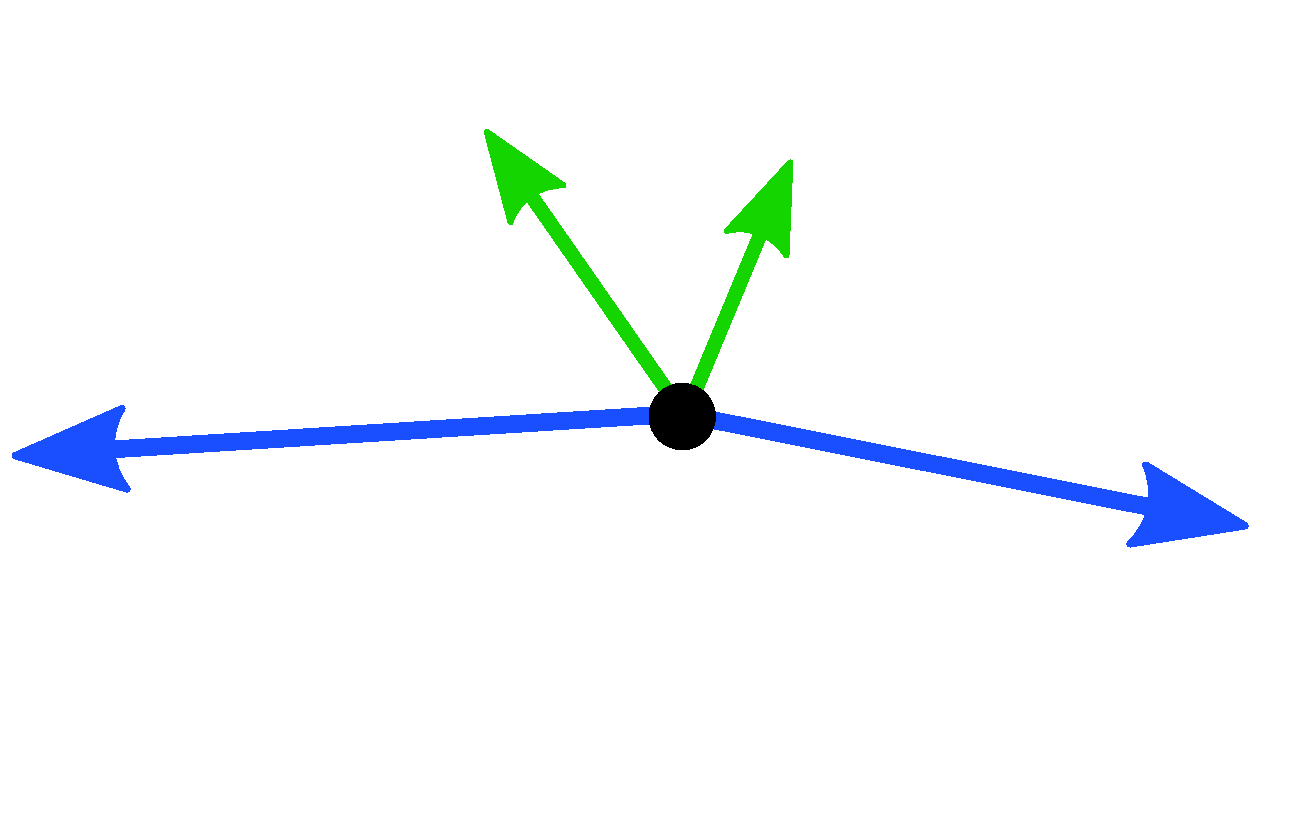
\includegraphics[width=\linewidth]{graphics/backgrounds/cep.pdf}}}
  \end{subfigure}
}%
\quad%
\parbox{0.315\textwidth}{%
  \centering%
  \begin{subfigure}[b]{0.9\linewidth}{
                \subcaptionbox{\label{fig:bkgdSources_cd}}{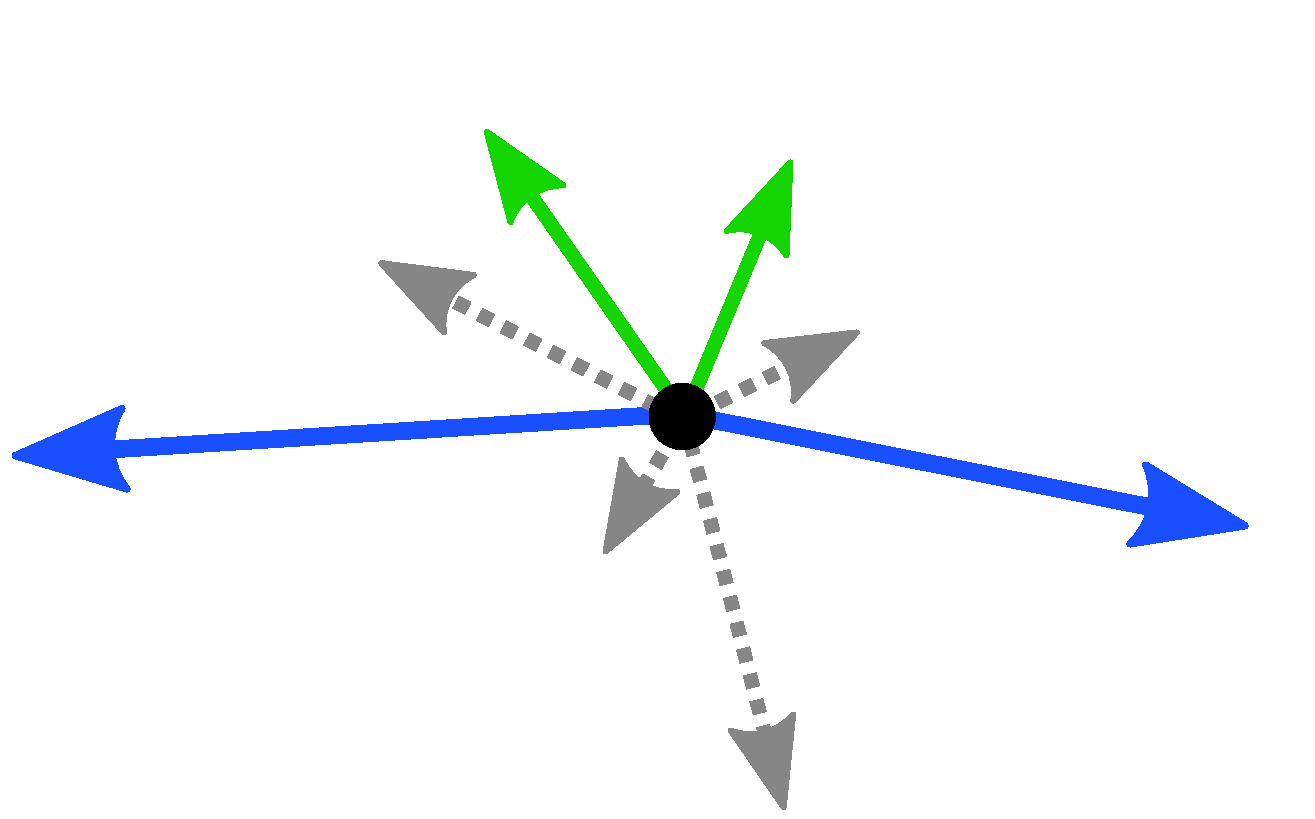
\includegraphics[width=\linewidth]{graphics/backgrounds/cd.pdf}}}
  \end{subfigure}
}%
\quad%
\parbox{0.315\textwidth}{%
  \centering%
  \begin{subfigure}[b]{0.9\linewidth}{
                \subcaptionbox{\label{fig:bkgdSources_mb_el}}{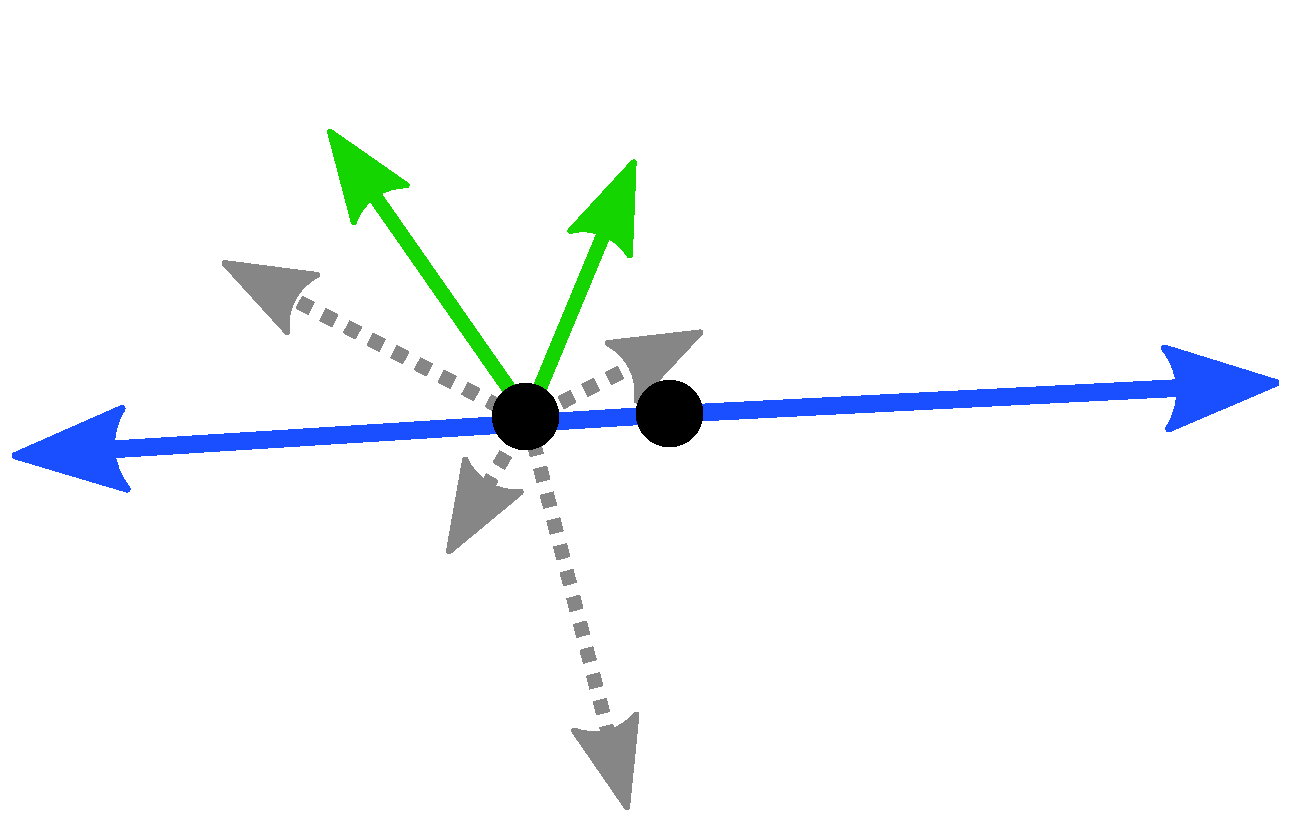
\includegraphics[width=\linewidth]{graphics/backgrounds/mb_el.pdf}}}
  \end{subfigure} 
}%
\caption[Sketches of main processes with CEP event topology.]{Sketches of main processes exhibiting $h^{+}h^{-}$ CEP event topology: the exclusive $h^{+}h^{-}$ signal itself (\subref{fig:bkgdSources_cep}), central diffraction event with some particles not detected (\subref{fig:bkgdSources_cd}) and elastic proton-proton scattering event with pile-up inelastic interaction in the central region (\subref{fig:bkgdSources_mb_el}). Particles represented by arrows are: forward scattered protons (blue), detected mid-rapidity particles (green) and undetected particles (dashed gray). Black dots mark primary interaction vertices.}\label{fig:bkgdSources}
\end{figure}
%---------------------------
 
 

% %---------------------------
% \begin{figure}[h]
% \centering%
% 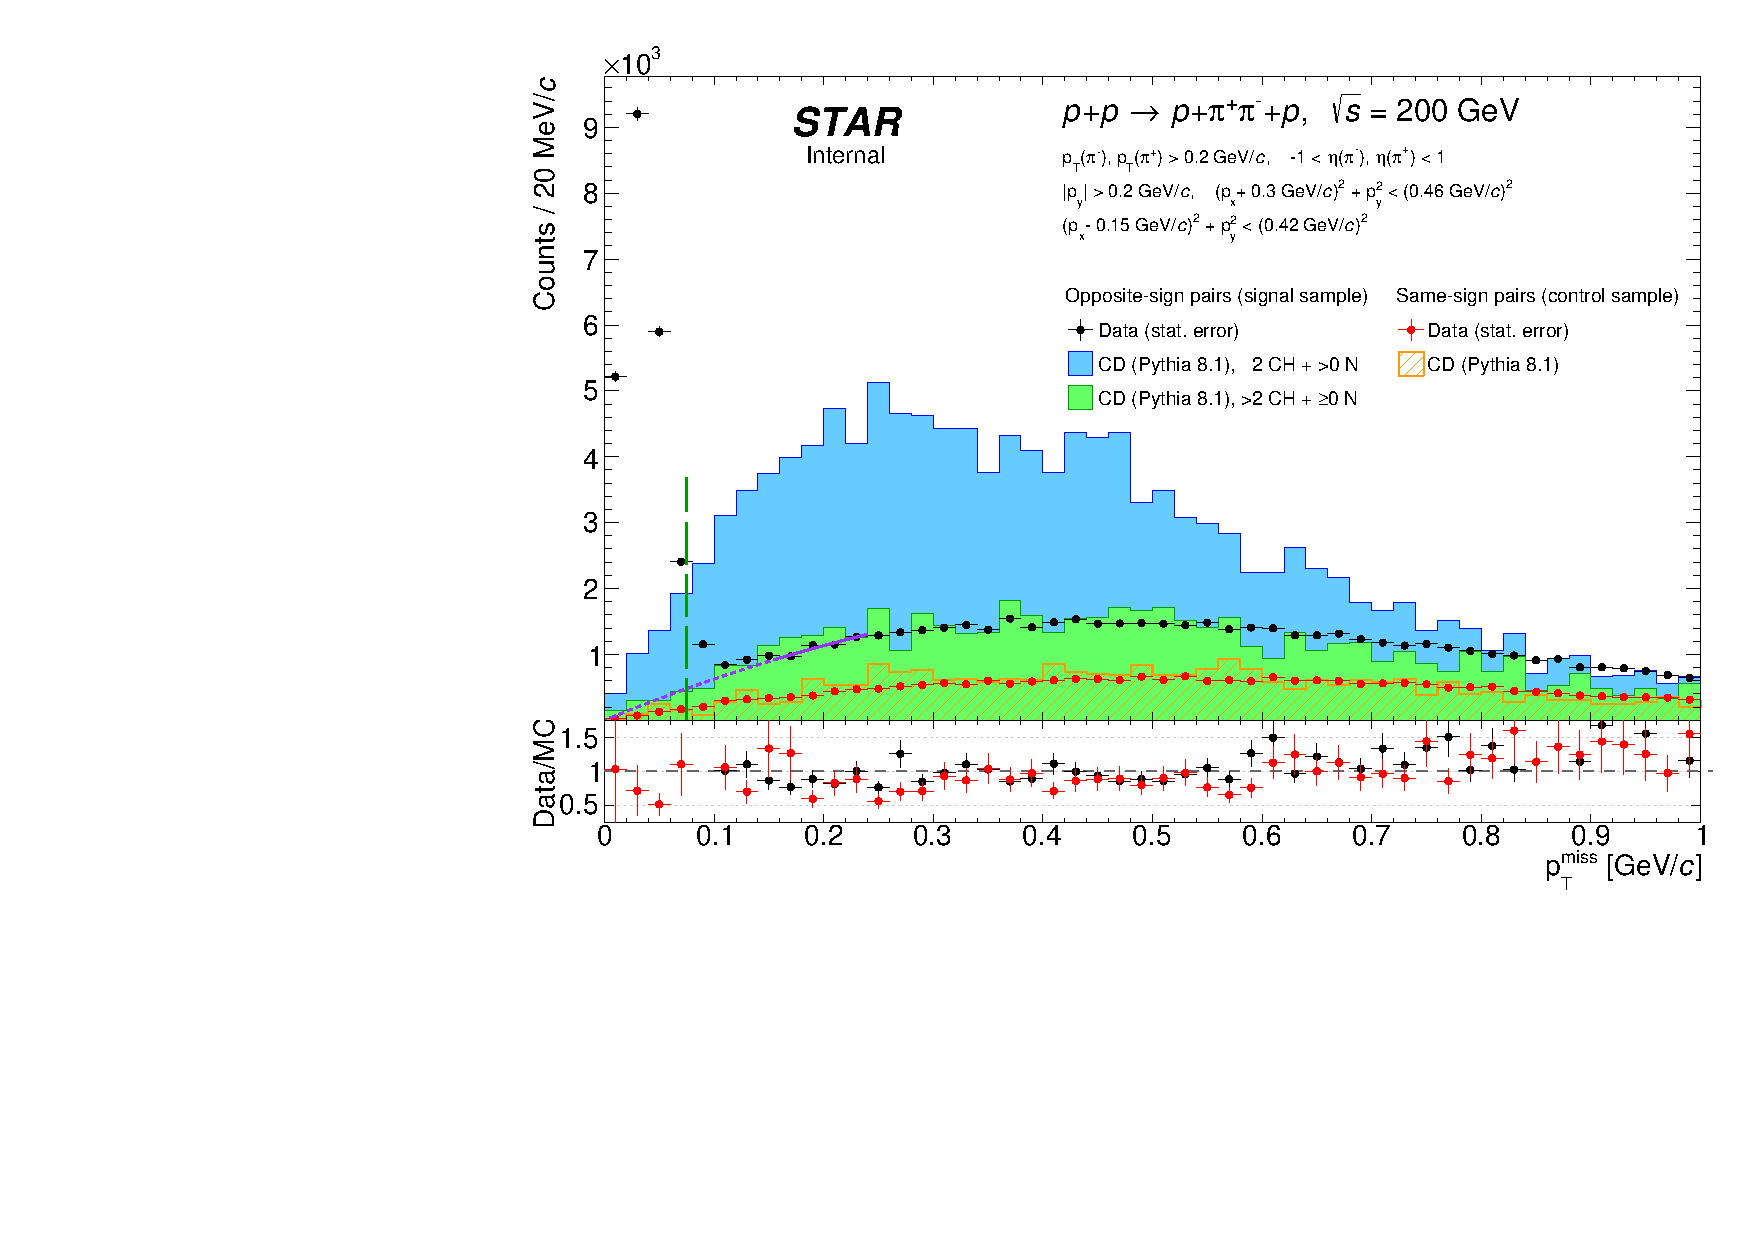
\includegraphics[width=0.65\linewidth,page=1]{graphics/backgrounds/Raw_MissingPtPid.pdf}%
% \caption{Missing pT.}\label{fig:missingPtBkgd}%
% \end{figure}
% %---------------------------
\newpage
\subsection{Exclusive background (particle misidentification)}\label{sec:exclBkgd}

Another source of background which is connected with finite particle identification power is the exclusive background from the particle species other than species under study. This effect is schematically shown in Fig.~\ref{fig:misidentificationGraph}, %
%---------------------------
\begin{figure}[h!]\vspace{5pt}
\centering%
\parbox{0.4725\textwidth}{%
  \centering%
  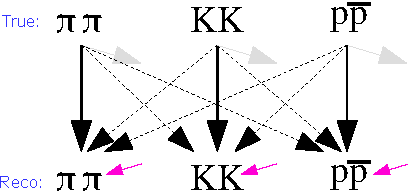
\includegraphics[width=\linewidth]{graphics/backgrounds/pid-crop2.pdf}
}%
\quad%
\parbox{0.4725\textwidth}{%
    \caption[Graph illustrating the misidentification problem.]{Graph illustrating the misidentification problem - the origin of exclusive background in selected samples. Gray arrows represent event rejection due to failed PID selection (\ref{enum:CutPid}). Magenta arrows indicate non-exclusive backgrounds described in Sec.~\ref{sec:nonExclBkgd}. Solid black arrows represent successful identification, whereas dashed black lines show misidentification paths.}\label{fig:misidentificationGraph}
}%
\vspace{5pt}
\end{figure}
%--------------------------- 
and written in the form of set of equations~\eqref{eq:misidentificationEqs}, where $N^{XX}_{R}$ is number of reconstructed events identified as $XX$ ($X=\pi, K \text{~or~} p$), $N^{XX}_{T}$ is true number of $XX$ events, $N^{\pi\pi}_{bkgd}$ is number of non-exclusive events among reconstructed $N^{XX}_{R}$, $\epsilon^{XX}$ is identification efficiency for species $XX$, and $\lambda^{XX\rightarrow YY}$ is misidentification probability of species $XX$ as $YY$ (see Sec.~\ref{sec:pidEff}):
\begin{subequations}\label{eq:misidentificationEqs}\vspace{5pt}
\begin{equation}
  N^{\pi\pi}_{R}~~=~~\begingroup\color{gray}\underbrace{\color{black}\epsilon^{\pi\pi}\cdot N^{\pi\pi}_{T}}_{\textrm{true pion pairs}}\endgroup~~ + ~~\begingroup\color{gray}\underbrace{\color{black}\lambda^{ KK\rightarrow \pi\pi}\cdot N^{KK}_{T}}_{\substack{\textrm{kaon pairs reconstructed} \\ \textrm{as pion pairs}}}\endgroup~~ + ~~\begingroup\color{gray}\underbrace{\color{black}\lambda^{p\bar{p} \rightarrow \pi\pi} \cdot N^{p\bar{p}}_{T}}_{\substack{\textrm{proton pairs reconstructed} \\ \textrm{as pion pairs}}}\endgroup~~ + ~~\textcolor{magenta}{N^{\pi\pi}_{bkgd}}
\end{equation}    
\begin{equation}
  N^{KK}_{R} ~= ~~\begingroup\color{gray}\underbrace{\color{black}\lambda^{ \pi\pi\rightarrow KK}\cdot N^{\pi\pi}_{T}}_{\substack{\textrm{pion pairs reconstructed} \\ \textrm{as kaon pairs}}}\endgroup~~ + ~~\begingroup\color{gray}\underbrace{\color{black}\epsilon^{KK}\cdot N^{KK}_{T}}_{\textrm{true kaon pairs}}\endgroup~~ + ~~\begingroup\color{gray}\underbrace{\color{black}\lambda^{p\bar{p} \rightarrow KK} \cdot N^{p\bar{p}}_{T}}_{\substack{\textrm{proton pairs reconstructed} \\ \textrm{as kaon pairs}}}\endgroup~~ + ~~\textcolor{magenta}{N^{KK}_{bkgd}}
\end{equation}
\begin{equation}\hspace*{-25pt}
  N^{p\bar{p}}_{R}~~~= ~~\begingroup\color{gray}\underbrace{\color{black}\lambda^{\pi\pi \rightarrow p\bar{p}} \cdot N^{\pi\pi}_{T}}_{\substack{\textrm{pion pairs reconstructed} \\ \textrm{as proton pairs}}}\endgroup~~ + ~~\begingroup\color{gray}\underbrace{\color{black}\lambda^{ KK\rightarrow p\bar{p}}\cdot N^{KK}_{T}}_{\substack{\textrm{kaon pairs reconstructed} \\ \textrm{as proton pairs}}}\endgroup~~ + ~~\begingroup\color{gray}\underbrace{\color{black}\epsilon^{p\bar{p}}\cdot N^{p\bar{p}}_{T}}_{\textrm{true proton pairs}}\endgroup~~ + ~~\textcolor{magenta}{N^{p\bar{p}}_{bkgd}}
\end{equation}\vspace{5pt}
\end{subequations}

We only consider three most significant possible hadronic CEP channels - next in a row would be CEP of $d\bar{d}$, but such events are not observed in the data, although reconstruction efficiency should be similar to $p\bar{p}$. Eqs.~\eqref{eq:misidentificationEqs} can be written in the matrix form, as shown in Eq.~\eqref{eq:misidentificationMatrix}, from which it is straightforward to obtain final formula for restored number of events of given ID, Eq.~\eqref{eq:pidUnfoldingMatrix}:

\begin{tabulary}{\textwidth}{LCL}
\begin{equation}\label{eq:misidentificationMatrix}\hspace*{-15pt}
\Spvek{N^{\pi\pi}_{R}-\textcolor{magenta}{N^{\pi\pi}_{bkgd}};~;N^{KK}_{R}-\textcolor{magenta}{N^{KK}_{bkgd}};~;N^{p\bar{p}}_{R}-\textcolor{magenta}{N^{p\bar{p}}_{bkgd}}} =  \underbrace{\left[ \begin{array}{ccc}
\epsilon^{\pi\pi} & \lambda^{ KK\rightarrow \pi\pi} & \lambda^{p\bar{p} \rightarrow \pi\pi} \\
~ & ~ & ~\\
\lambda^{\pi\pi\rightarrow KK} & \epsilon^{KK} & \lambda^{ p\bar{p} \rightarrow KK}\\
~ & ~ & ~\\
\lambda^{\pi\pi\rightarrow p\bar{p}} & \lambda^{ KK\rightarrow p\bar{p}} & \epsilon^{p\bar{p}}
\end{array} \right]}_{\text{``mixing matrix''}~\Lambda}\Spvek{N^{\pi\pi}_{T};~;N^{KK}_{T};~;N^{p\bar{p}}_{T}}
\end{equation}&%
\vspace{40pt}$\rightarrow$\hspace{20pt}&
\begin{equation}\label{eq:pidUnfoldingMatrix}
\Spvek{N^{\pi\pi}_{T};~;N^{KK}_{T};~;N^{p\bar{p}}_{T}} = \Lambda^{-1}\Spvek{N^{\pi\pi}_{R}-\textcolor{magenta}{N^{\pi\pi}_{bkgd}};~;N^{KK}_{R}-\textcolor{magenta}{N^{KK}_{bkgd}};~;N^{p\bar{p}}_{R}-\textcolor{magenta}{N^{p\bar{p}}_{bkgd}}}
\end{equation}
\end{tabulary}

In Sec.~\ref{sec:exclBkgdDetermination} we show a semi-data-driven method of estimation of the exclusive background.
 
 
\section{Background determination} 
\subsection{Non-exclusive background}\label{sec:nonExclBkgdDetermination}

Determination of non-exclusive background makes use of the missing transverse momentum which is distributed differently for the signal and for aforementioned background. High statistics of the data allows to apply a data-driven method, which is desired as it does not introduce model-dependence to results, especially when models of diffraction do not describe physics observables. What is more, not only integrated over observables but differentially as a function of these.

It has already been demonstrated in Sec.~\ref{subsec:ptMiss} that $p_{\text{T}}^{\text{miss}}$ from exclusive events is much narrower compared to background, visible as a peak near the axis origin. Additional feature of 
$p_{\text{T}}^{\text{miss}}$ - probability density approaching to zero with $p_{\text{T}}^{\text{miss}}$ moving towards the axis origin, helps performing a polynomial fit without constant component to $p_{\text{T}}^{\text{miss}}$ distribution in the background-dominated range and extrapolation of this polynomial down to $p_{\text{T}}^{\text{miss}} = 0$ under the peak of CEP signal. The procedure used to determine non-exclusive background content in the signal region is described below. The description assumes determination of non-exclusive background differentially in single observable $X$ (in 1 dimension), but procedure naturally applies also to more dimensions.

\begin{enumerate}
 \item 2-dimensional distribution of $p_{\text{T}}^{\text{miss}}$ vs. $X$ (by design without cut~\ref{enum:CutMissingPt} applied) was looped over all bins in $X$. Projection onto $p_{\text{T}}^{\text{miss}}$ axis, $\frac{dN_{X}}{dp_{T}^{\text{miss}}}$, was done for only these bins of $X$, in which there are signal candidates (more than 0 counts in the region $p_{\text{T}}^{\text{miss}}<75$~MeV).
 \item Projections of $p_{\text{T}}^{\text{miss}}$ from bins with signal candidates are summed to a single histogram (like data points in Fig.~\ref{fig:nonExclBkgdDetermination}):
 \begin{equation}
  \frac{dN}{dp_{T}^{\text{miss}}} = \sum_{X}\frac{dN_{X}}{dp_{T}^{\text{miss}}}
 \end{equation}

 \item Fit of polynomial given by Eq.~\eqref{eq:polynomial} was performed to $\frac{dN}{dp_{T}^{\text{miss}}}$ in the range $160~\text{MeV}<p_{\text{T}}^{\text{miss}}<240~\text{MeV}$, where dominant non-exclusive background with negligibly low signal content is expected.
 \begin{equation}\label{eq:polynomial}
 b\left(p_{T}^{\text{miss}}\right) = c_{1}\cdot p_{T}^{\text{miss}} + c_{2}\cdot\left(p_{T}^{\text{miss}}\right)^2
\end{equation}
The left egde of the fitting range was chosen to be close to $p_{\text{T}}^{\text{miss}}=0$, but far enough from the signal peak which could bias fitted background shape. The right egde of the fitting range was set to provide reasonable width of that range, but on the other hand be close enough to $p_{\text{T}}^{\text{miss}}=0$, so that $2^{\text{nd}}$ order polynomial approximation would still be valid for the background shape. Result of the fit is shown in Fig.~\ref{fig:nonExclBkgdDetermination} with semi-transparent magenta line.
\item Ratio $r_{\text{bkgd}}$ was calculated between the integral of function $b$ in the signal region ($p_{\text{T}}^{\text{miss}}<75$~MeV)) and in the fitted region $160~\text{MeV}<p_{\text{T}}^{\text{miss}}<240~\text{MeV}$:
\begin{equation}\label{eq:r_bkgd}
 r_{\text{bkgd}} = \frac{\int\limits_{0}^{75~\text{MeV}} b\left(p_{T}^{\text{miss}}\right) dp_{T}^{\text{miss}}}{\int\limits_{160~\text{MeV}}^{240~\text{MeV}} b\left(p_{T}^{\text{miss}}\right) dp_{T}^{\text{miss}}}.
\end{equation}
\item In each bin of $X$ with any signal counts the non-exclusive background was determined as
\begin{equation}\label{eq:nonExclBkgd}
 N_{\text{bkgd},X}^{\text{non-excl}} = r_{\text{bkgd}} \cdot \int\limits_{0}^{75~\text{MeV}} \frac{dN_{X}}{dp_{T}^{\text{miss}}} dp_{T}^{\text{miss}}.
\end{equation}
\end{enumerate}

%---------------------------
\begin{figure}[ht!]
\centering%
\parbox{0.4725\textwidth}{%
  \centering%
  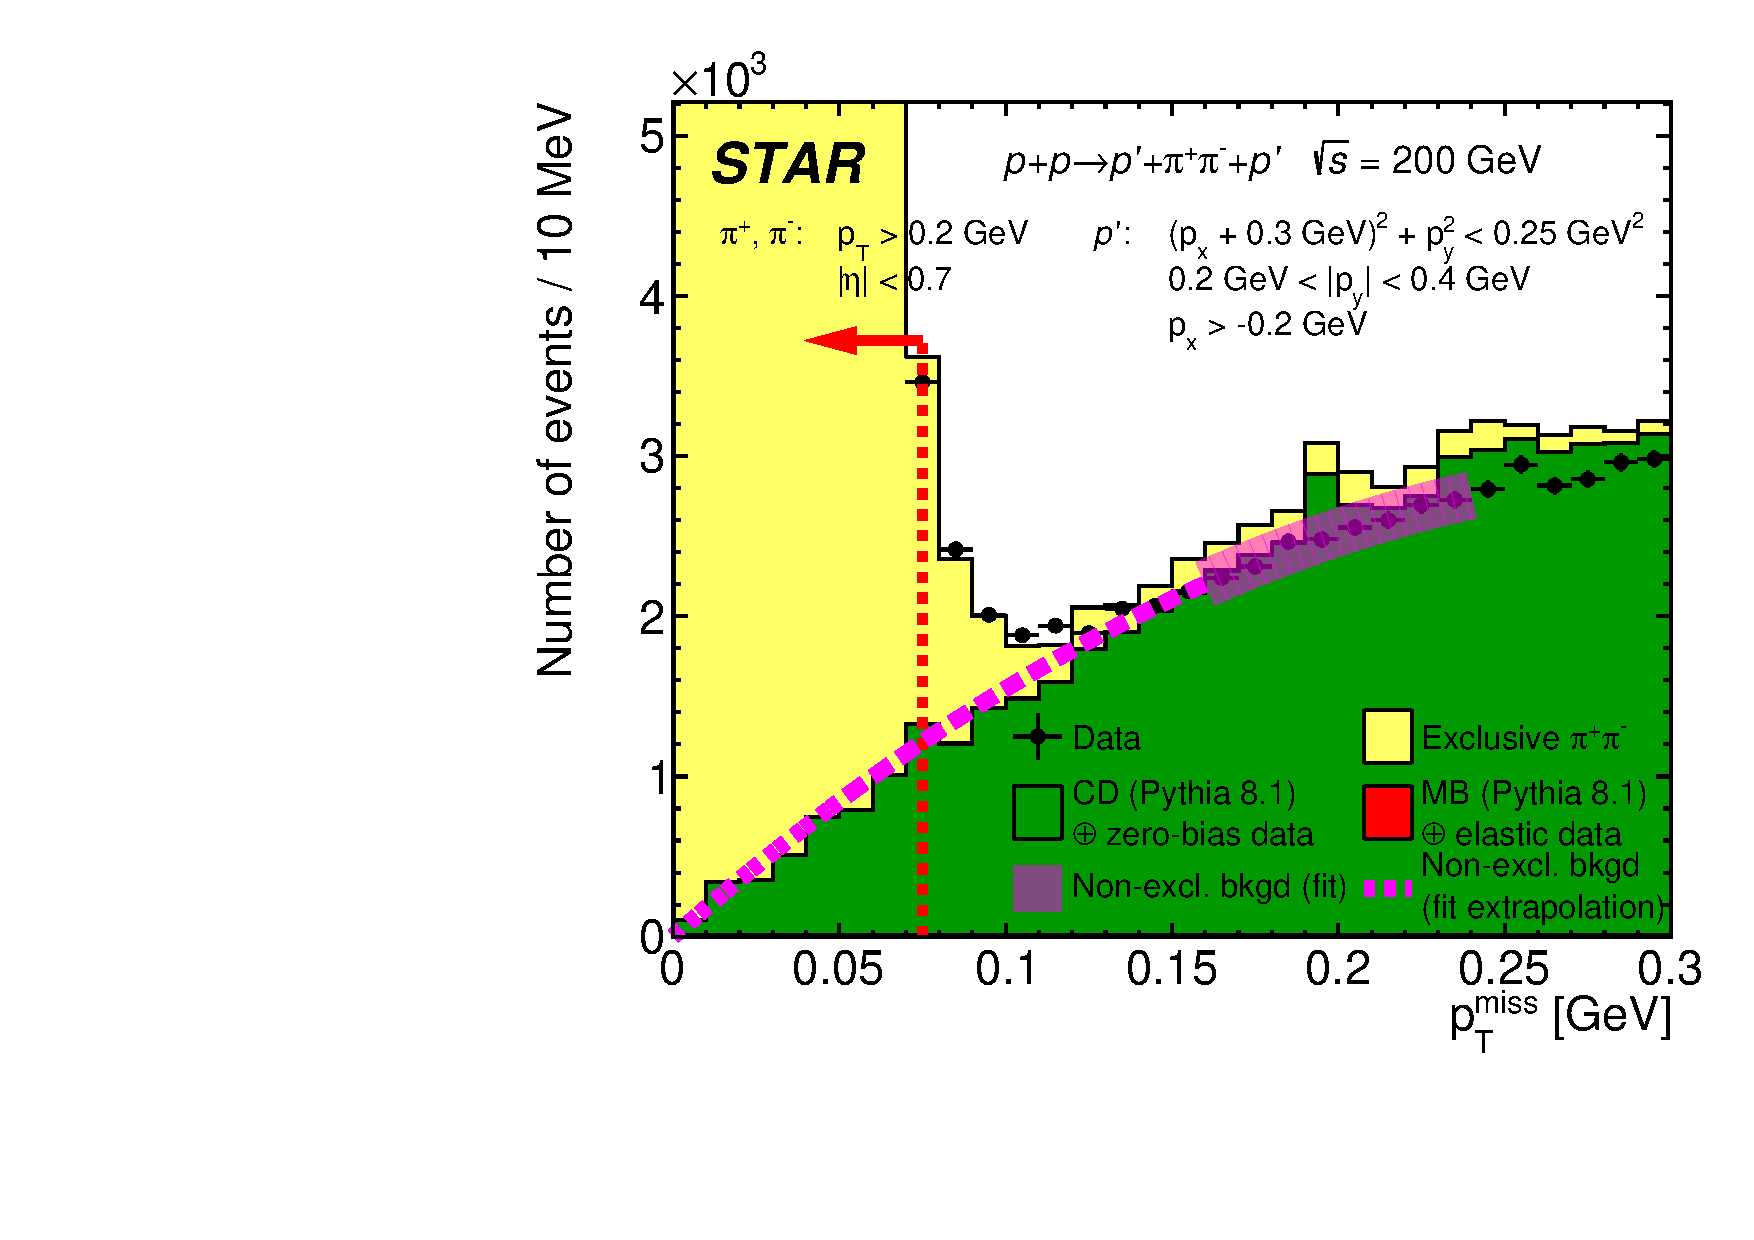
\includegraphics[width=\linewidth]{graphics/backgrounds/MissingPt_NonExclBkgdFitDemonstration.pdf} 
}%
\quad%
\parbox{0.4725\textwidth}{%
    \caption[Demonstration of non-exclusive background determination method using $p_{T}^{\text{miss}}$ distribution.]{Demonstration of non-exclusive background determination method using $p_{T}^{\text{miss}}$ distribution. Both data and MC predictions presented in the figure are the same as in Fig.~\ref{fig:Ratio_MissingPt} - here same sign events were ommited, as well as the binning was set finer and axes ranges were adjusted to focus on the background region below the signal peak. Normalization of MC components was explained in Sec.~\ref{sec:bkgdSignalNorm}. The data are shown with black points, stacked MC predictions are shown with filled histograms, and fit of $2^{\text{nd}}$ order polynomial given by Eq.~\eqref{eq:polynomial} representing non-exclusive background, together with its extrapolation to $p_{T}^{\text{miss}}=0$ is drawn with solid and dashed magenta line, respectively.}\label{fig:nonExclBkgdDetermination}%  
}
\end{figure}
%---------------------------


One can see in Fig.~\ref{fig:nonExclBkgdDetermination} that fitted polynomial extrapolated to $p_{\text{T}}^{\text{miss}}=0$ matches well predictions from MC. We conservatively estimate possible systematic under/overestimation of the non-exclusive background under the exclusive events peak to $\pm 10\%$, which we use in the systematic errors study presented in Sec.~\ref{sec:systEffectsList}.

In Fig.~\ref{fig:Ratio_InvMass} we demonstrate, that data driven method is necessary to obtain unbiased shape of the background - differences between MC predictions and data-driven estimates can be as high as 50\% both ways. Also, shape of the same-sign background is significantly different from opposite-sign estimate, which disqualifies usage of same-sign background as an estimate of non-exclusive opposite-sign background.


%---------------------------
\begin{figure}[ht!]
\centering%
\parbox{0.5725\textwidth}{%
  \centering%
  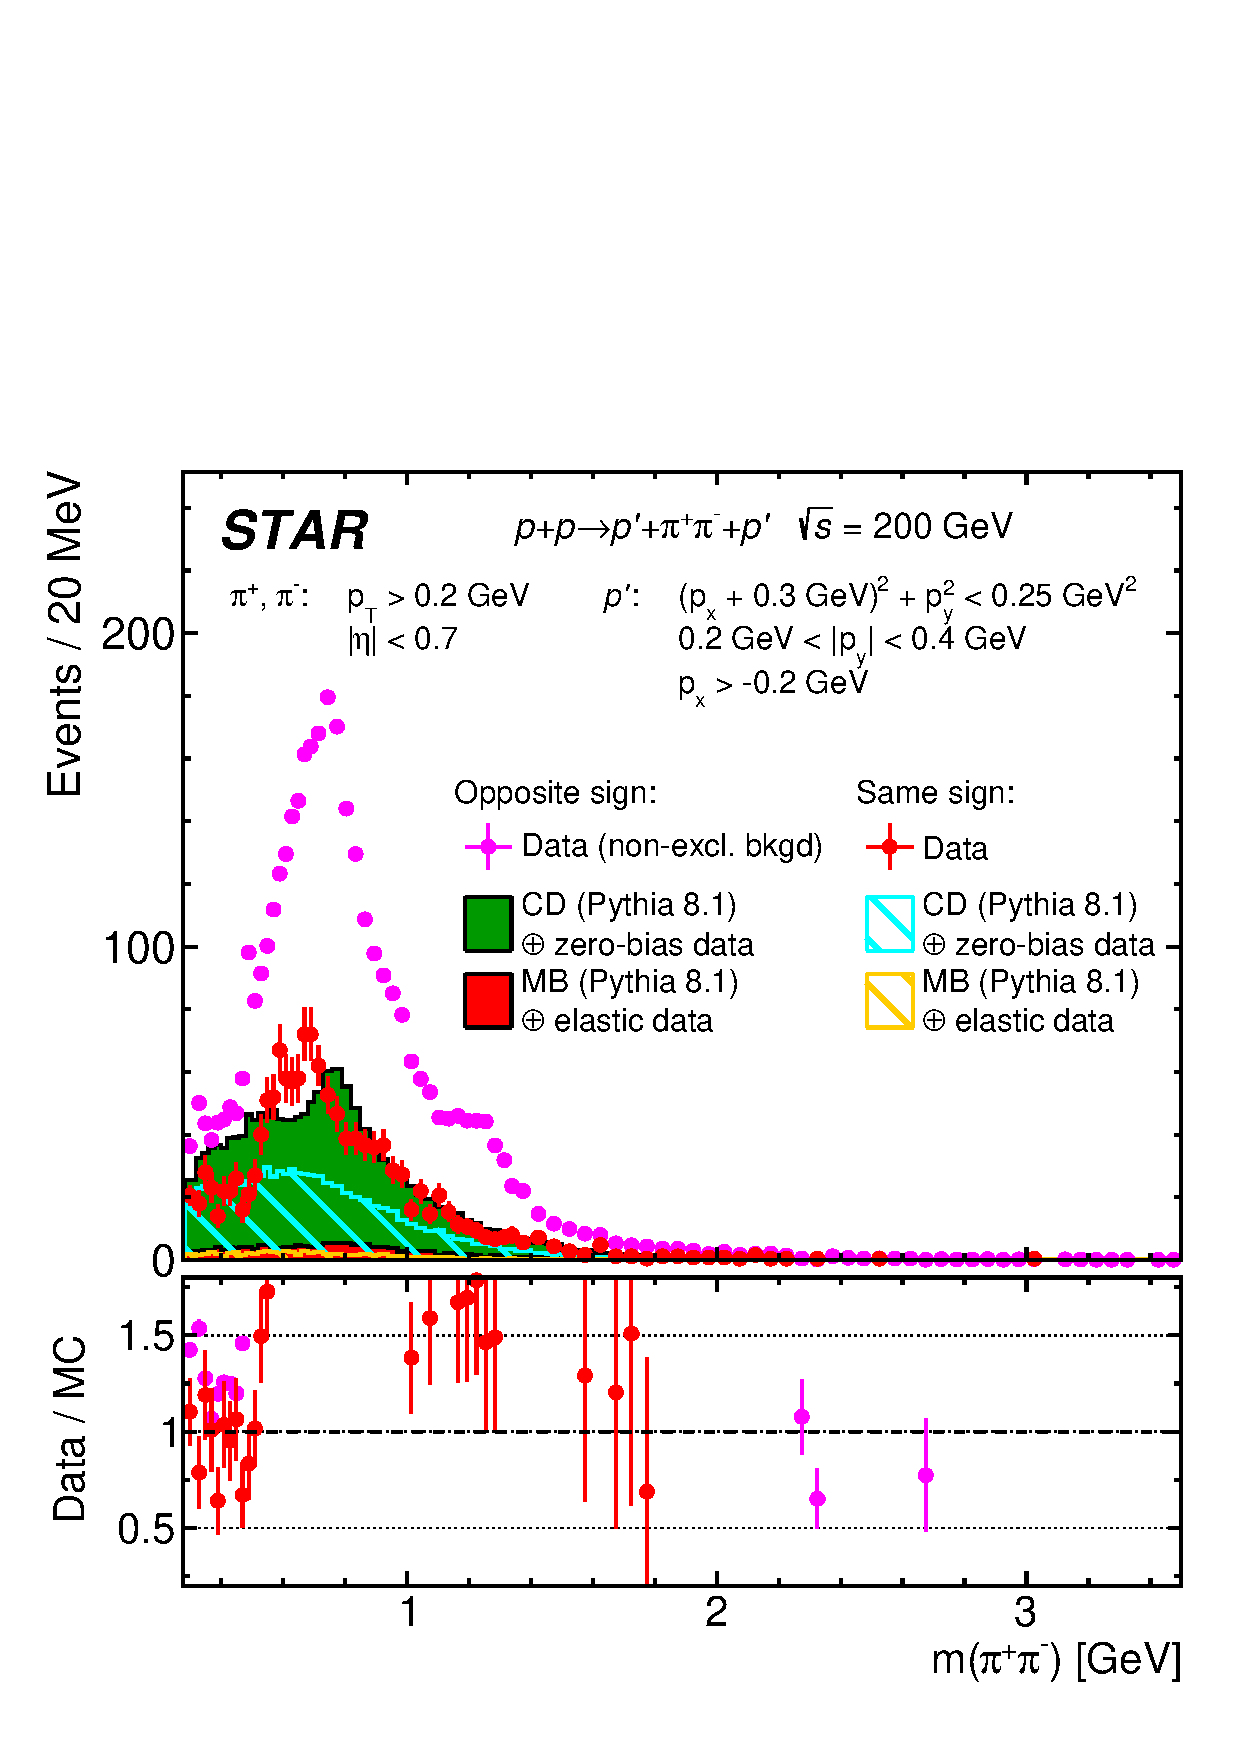
\includegraphics[width=\linewidth]{graphics/backgrounds/dataVsMc/Ratio_InvMass.pdf} 
}%
\quad%
\parbox{0.3725\textwidth}{%
    \caption[Comparison of non-exclusive background as a function of $m(\pi\pi)$ exctracted from data and MC predictions.]{Comparison of non-exclusive background as a function of $m(\pi\pi)$ exctracted from data and MC predictions. All offline selections were applied. Normalization of MC components was explained in Sec.~\ref{sec:bkgdSignalNorm}. Opposite-sign non-exclusive background extracted from data is shown with magneta points, while stacked opposite-sign MC predictions are shown with filled histograms. Control same-sign background events are shown with red points for the data, and stacked hatched histograms for MC predictions.}\label{fig:Ratio_InvMass} %  
}
\end{figure}
%---------------------------







\subsection{Exclusive background}\label{sec:exclBkgdDetermination}

Exclusive background arising from wrong identification have been estimated with the help of semi-data-driven method. This method uses fast MC generator introduced in Sec.~\ref{sec:pidEff}, in which all quantities relevant for particle identification ($dE/dx$ and its resolution, TOF time measurement resolution etc.) were set according to their distribution/magnitude in the data. In order to determine absolute size of migrations between three measured species of particle pairs it was required to know the full distribution of particles' (transverse) momenta - especially in the regions of momentum space where the migrations are significant (regions of non-zero $\lambda^{X\rightarrow Y}$ in Fig.~\ref{fig:pidEffVsPt}). There are no models of CEP of $\pi^{+}\pi^{-}$, $K^{+}K^{-}$ and $p\bar{p}$ which describe measured data, therefore we decided to use measured distributions as an input models of $(p_{T}^{+}, p_{T}^{-})$\footnote{$(p_{T}^{\text{max}}, p_{T}^{\text{min}})$ could be used same well.}. We assumed that selected CEP pairs have low contamination from the exclusive background (we know that non-exclusive is less than 7\%) and thus $(p_{T}^{+}, p_{T}^{-})$ distributions are representative for all particle species. Such assumption was motivated by restrictive particle identification algorithm, which based on study from Sec.~\ref{sec:pidEff} provides high level of identification efficiency and low level of misidentification probability. Also, in the distributions of $\chi^{2}_{dE/dx}$ and $m^{2}_{\text{TOF}}$ presented in Fig.~\ref{fig:pid_plots} we see clear features expected for given pair types, without signs of excessful exclusive background. Having commented that, raw distributions of $(p_{T}^{+}, p_{T}^{-})$ for selected CEP events without additional lower track $p_{T}$ cut~\ref{enum:CutPidPtLimits} for kaon and proton pairs (Figs.~\ref{fig:PtPlusVsPtMinus_pion_1}, \ref{fig:PtPlusVsPtMinus_kaon_1} and~\ref{fig:PtPlusVsPtMinus_proton_1}) were assumed to properly represent corresponding detected, reconstructed and identified particle species.

The following procedure was conducted to prepare $(p_{T}^{+}, p_{T}^{-})$ distributions finally used to determine exclusive background in all three CEP samples:

\begin{enumerate}
 \item Distributions exhibit natural symmetry around $p_{T}^{+}=p_{T}^{-}$ therefore corresponding mirror-image bins with respect to diagonal were averaged:
 \begin{equation}
  N_{X,avg}(p_{T}^{+}, p_{T}^{-}) = N_{X,avg}(p_{T}^{-}, p_{T}^{+}) = \frac{N_{X}(p_{T}^{-}, p_{T}^{+}) + N_{X}(p_{T}^{+}, p_{T}^{-})}{2}.
 \end{equation}
Outcome for all three species is shown in Figs.~\ref{fig:PtPlusVsPtMinus_pion_2}, \ref{fig:PtPlusVsPtMinus_kaon_2} and~\ref{fig:PtPlusVsPtMinus_proton_2}.
 \item Distributions were corrected for the identification efficiency from Fig.~\ref{fig:pidEffVsPt}:
 \begin{equation}
  N_{X,corr}(p_{T}^{+}, p_{T}^{-}) = \frac{N_{X,avg}(p_{T}^{-}, p_{T}^{+})}{ \mbox{\LARGE$\epsilon$}^{X}\left(max(p_{T}^{-}, p_{T}^{+}), min(p_{T}^{-}, p_{T}^{+})\right) }.
 \end{equation}
 At this stage distributions $N_{X,corr}$ represent detected and reconstructed events before identification. They are drawn in Figs.~\ref{fig:PtPlusVsPtMinus_pion_3}, \ref{fig:PtPlusVsPtMinus_kaon_3} and~\ref{fig:PtPlusVsPtMinus_proton_3}.
 \item Last step of preparation of $(p_{T}^{+}, p_{T}^{-})$ distributions applies only to $K^{+}K^{-}$ and $p\bar{p}$, as it is related with the upper cut on $min(p_{T}^{-}, p_{T}^{+})$. Because of this cut we do not have acces to region where both-tracks' carry high $p_{T}$. We overcome this difficulty by performing an extrapolation of the distributions into the unmeasured region. This is done for the histograms binned as shown in figures mentioned earlier. In a loop over all bins in $p_{T}^{-}$ (index $i$) and in $p_{T}^{+}$ (index $j$) the following prescription is used to fill empty bins, starting from the bins covering $min(p_{T}^{-}, p_{T}^{+})$ cuts specific for $K^{+}K^{-}$ and $p\bar{p}$:
 \begin{equation}
  N_{X,extr}(p_{T,i}^{+}, p_{T,j}^{-}) = f_{extr}\cdot\frac{N_{X,extr}(p_{T,i-1}^{-}, p_{T,j-1}^{+}) + N_{X,extr}(p_{T,i-2}^{+}, p_{T,j-2}^{-})}{2}.
 \end{equation}
In above furmula factor $f_{extr}$ determines the ``steepnes'' of the distribution with growing track's $p_{T}$. As we observe in $\pi^{+}\pi^{-}$ channel the high-$p_{T}$ tail in the distribution tends to diminish and disappears around $(2~\text{GeV}, 2~\text{GeV})$. We find that $f_{extr}=0.8$ is reasonable to provide picture similar to $\pi^{+}\pi^{-}$ in the two remaining CEP channels. Final distributions for $K^{+}K^{-}$ and $p\bar{p}$ are drawn in Figs.~\ref{fig:PtPlusVsPtMinus_kaon_4} and~\ref{fig:PtPlusVsPtMinus_proton_4}, respectively.
\end{enumerate}

Prepared $(p_{T}^{+}, p_{T}^{-})$ distributions were used to obtain predictions for the misidentifications. Samples of exclusive $\pi^{+}\pi^{-}$, $K^{+}K^{-}$ and $p\bar{p}$ simulated with fast MC, with uniformly distributed $(p_{T}^{+}, p_{T}^{-})$ over $0.2~\text{GeV}<p_{T}^{+}, p_{T}^{-}<3~\text{GeV}$, were subjected to PID algorithm~\ref{enum:CutPid}. Each event was assigned with the weight equal to the data-extracted event density for given $(p_{T}^{+}, p_{T}^{-})$, such that relative number of $\pi^{+}\pi^{-}$, $K^{+}K^{-}$ and $p\bar{p}$ pairs was exactly the same as it resulted from $(p_{T}^{+}, p_{T}^{-})$ maps in Fig.~\ref{fig:PtPlusVsPtMinus_pion_3}, \ref{fig:PtPlusVsPtMinus_kaon_4} and~\ref{fig:PtPlusVsPtMinus_proton_4}. Histograms of $\chi^{2}_{dE/dx}$ and $m^{2}_{\text{TOF}}$ were filled with reconstructed quantities and using aforementioned weight. There were were seperate histograms for different true-level PIDs and reconstructed PIDs, so that they formed $3\times3$ array of histograms.

The last step involved proper normalization of the histograms obtained earlier. Predictions for each true-level pair type were normalized independently, but the same normalization was preserved for all quantities and for all reconstructed pair types. Normalization $F^{\text{MC}}_{X}$ of histograms representing prediction for exclusive $XX$ was established such that the number of predicted $XX$ events in the $XX$ signal-dominating region (fiducial region of $\chi^{2}_{dE/dx}(XX)<6$), $N_{X\rightarrow X, \text{fid}}^{\text{MC}}$, was equal to the number of measured $XX$ events in that region ($N_{X,\text{fid}}^{\text{data}}$) less a number of non-exclusive background events in the same region ($N_{\text{bkgd},X,\text{fid}}^{\text{non-excl}}$) extracted with a method introduced in Sec.~\ref{sec:nonExclBkgdDetermination}. It is expressed with the formula in Eq.~\eqref{eq:exclBkgdNorm}:

\begin{equation}\label{eq:exclBkgdNorm}
 F_{X}^{\text{MC}} = \frac{ N_{X,\text{fid}}^{\text{data}} - N_{\text{bkgd},X,\text{fid}}^{\text{non-excl}} }{ N_{X\rightarrow X, \text{fid}}^{\text{MC}} }
\end{equation}% 
%
where all components are excplicitly given in Eqs.~\eqref{eq:exclBkgdNorm_1}-\eqref{eq:exclBkgdNorm_3}:\newline
%
\begin{tabulary}{\textwidth}{LCR}
\begin{equation}\label{eq:exclBkgdNorm_1}\hspace*{-2pt}
	 N_{\text{bkgd},X,\text{fid}}^{\text{non-excl}} = \int\limits_{0}^{6}\frac{dN_{\text{bkgd},X,\text{fid}}^{\text{non-excl}}}{d\chi^{2}_{dE/dx}}d\chi^{2}_{dE/dx},
\end{equation}&
\begin{equation}\label{eq:exclBkgdNorm_2}~~~~~~~
	N_{X,\text{fid}}^{\text{data}} = \int\limits_{0}^{6}\frac{dN_{X}^{\text{data}}}{d\chi^{2}_{dE/dx}}d\chi^{2}_{dE/dx},
\end{equation}&
\begin{equation}\label{eq:exclBkgdNorm_3}\hspace*{10pt}
	N_{X\rightarrow X, \text{fid}}^{\text{MC}} = \int\limits_{0}^{6}\frac{dN_{X\rightarrow X}^{\text{MC}}}{d\chi^{2}_{dE/dx}}d\chi^{2}_{dE/dx}.
\end{equation}
\end{tabulary}%

The relation between resultant normalization factors $F_{\pi\pi}^{\text{MC}}/F_{KK}^{\text{MC}}/F_{pp}^{\text{MC}}$ amounts 1/1.01/0.88. Comparisons of the data with the fast MC predictions normalized according above prescription are shown in Fig.~\ref{fig:pid_plots}. Fast MC well reproduces measured spectra of $\chi^{2}_{dE/dx}$ and $m^{2}_{\text{TOF}}$ for all selected particle pair species.


\begin{figure}[h]
\centering
\parbox{0.4725\textwidth}{
  \centering
  \begin{subfigure}[b]{\linewidth}
                \subcaptionbox{\label{fig:PtPlusVsPtMinus_pion_1}}{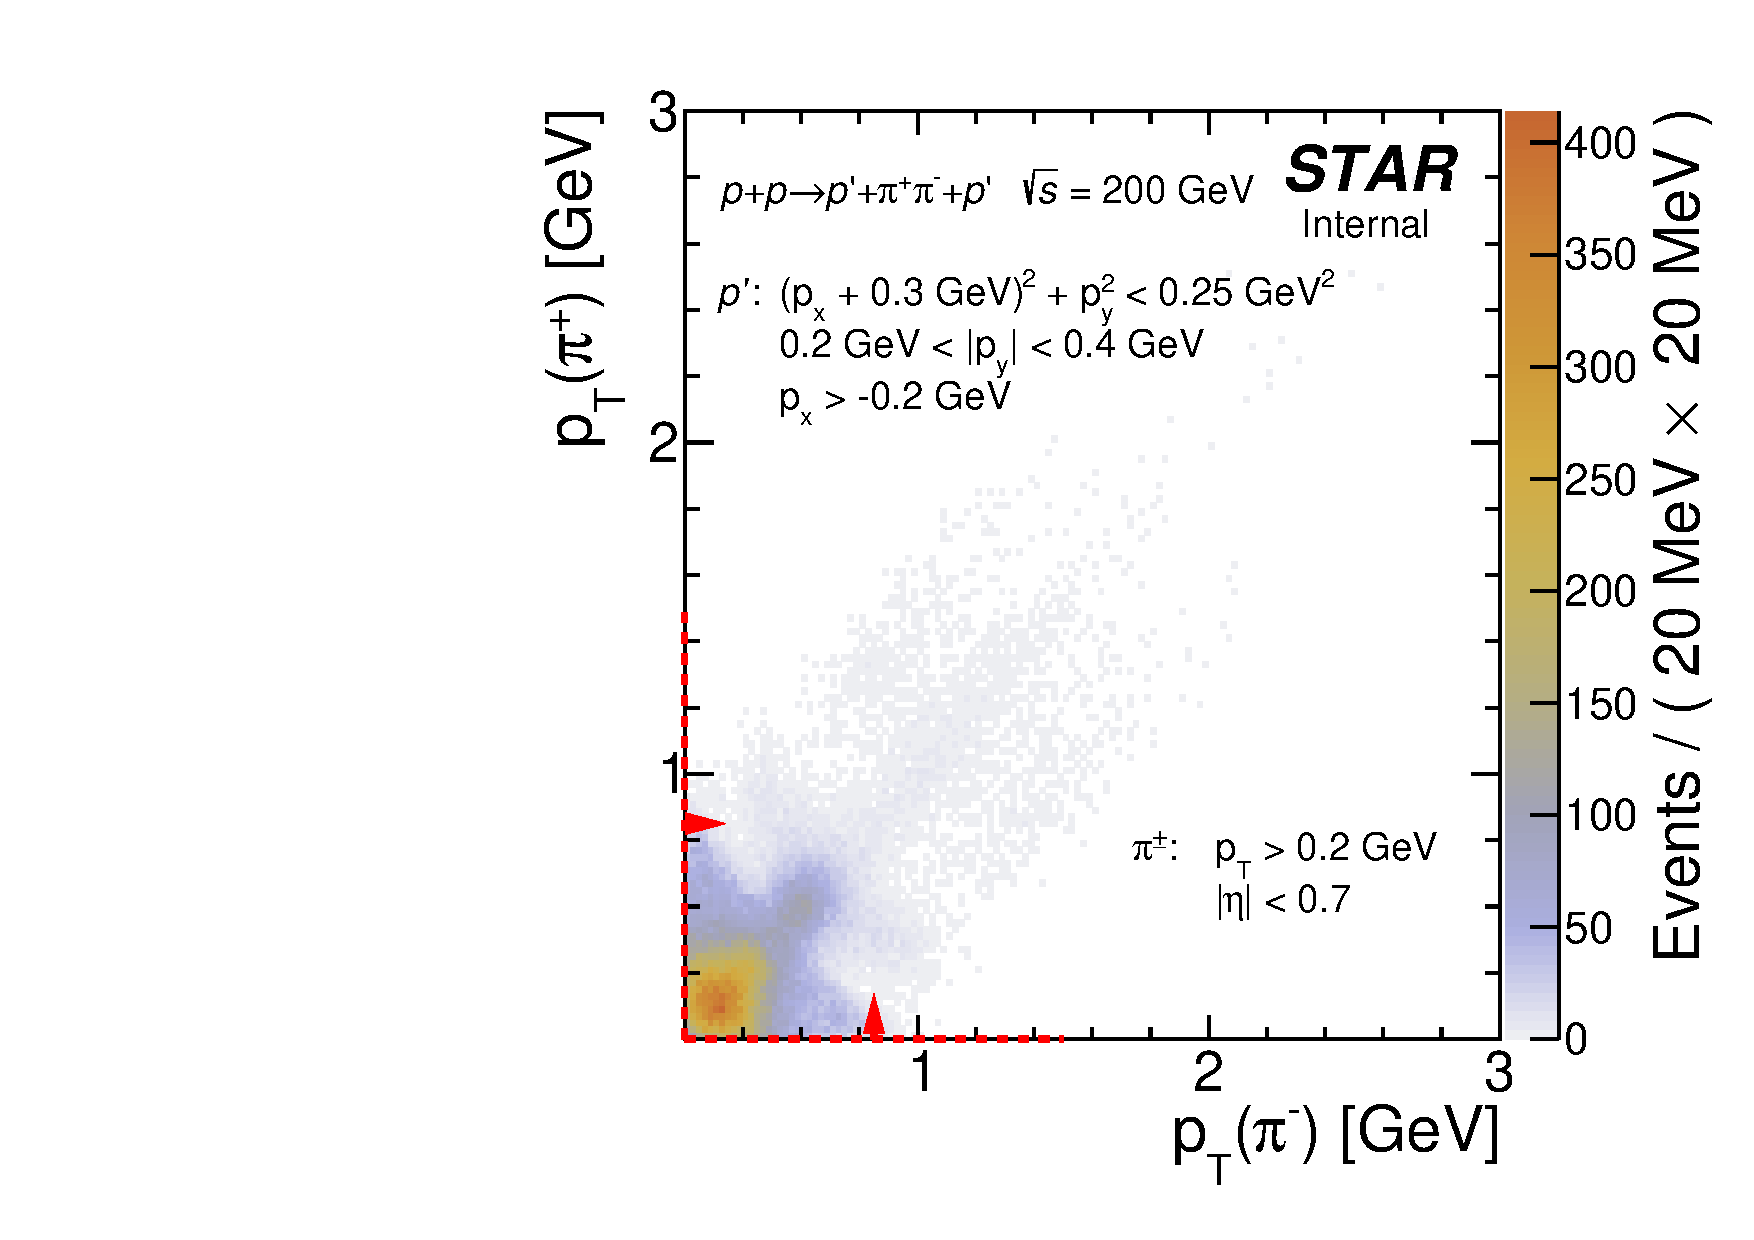
\includegraphics[width=1.05\linewidth,page=1]{graphics/backgrounds/exclusive/PtPlusVsPtMinusPid.pdf}}
  \end{subfigure}\\
  \begin{subfigure}[b]{\linewidth}\addtocounter{subfigure}{1}
                \subcaptionbox{\label{fig:PtPlusVsPtMinus_pion_3}}{\includegraphics[width=1.05\linewidth,page=3]{graphics/backgrounds/exclusive/PtPlusVsPtMinusPid.pdf}}
  \end{subfigure} 
}%
\quad\quad%
\parbox{0.4725\textwidth}{
  \centering
  \begin{subfigure}[b]{\linewidth}\addtocounter{subfigure}{-2}\vspace*{-10pt}
                \subcaptionbox{\label{fig:PtPlusVsPtMinus_pion_2}}{\includegraphics[width=1.05\linewidth,page=2]{graphics/backgrounds/exclusive/PtPlusVsPtMinusPid.pdf}}
  \end{subfigure}\\
  \begin{minipage}[t][1.042\linewidth][t]{\linewidth}\vspace{10pt}
    \caption[Two-dimensional distribution of positive and negative track transverse momentum for CEP $\pi^{+}\pi^{-}$ events.]{Two-dimensional distribution of positive and negative track transverse momentum for CEP events with TPC tracks identified as $\pi^{+}\pi^{-}$ pair. In Fig.~\subref{fig:PtPlusVsPtMinus_pion_1} original, raw distribution is shown. In Fig.~\subref{fig:PtPlusVsPtMinus_pion_2} distribution after symmetrization (averaging with respect diagonal) is drawn. Fig.~\subref{fig:PtPlusVsPtMinus_pion_3} shows symmetrized distribution additionally bin-by-bin corrected for pion pair identification efficiency shown in Fig.~\ref{fig:pidEffVsPt}a. Dashed red lines and arrows mark cut on tracks transverse momenta finaly used in physics analysis of CEP of $\pi^{+}\pi^{-}$ pairs.}\label{fig:PtPlusVsPtMinus_pion}
  \end{minipage}
}%
\end{figure}
%--------------------------- 


\begin{figure}[h]
\centering
\parbox{0.4725\textwidth}{
  \centering
  \begin{subfigure}[b]{\linewidth}
                \subcaptionbox{\label{fig:PtPlusVsPtMinus_kaon_1}}{\includegraphics[width=1.05\linewidth,page=4]{graphics/backgrounds/exclusive/PtPlusVsPtMinusPid.pdf}}
  \end{subfigure}\\
  \begin{subfigure}[b]{\linewidth}\addtocounter{subfigure}{1}
                \subcaptionbox{\label{fig:PtPlusVsPtMinus_kaon_3}}{\includegraphics[width=1.05\linewidth,page=6]{graphics/backgrounds/exclusive/PtPlusVsPtMinusPid.pdf}}
  \end{subfigure} 
}%
\quad\quad%
\parbox{0.4725\textwidth}{
  \centering
  \begin{subfigure}[b]{\linewidth}\addtocounter{subfigure}{-2}
                \subcaptionbox{\label{fig:PtPlusVsPtMinus_kaon_2}}{\includegraphics[width=1.05\linewidth,page=5]{graphics/backgrounds/exclusive/PtPlusVsPtMinusPid.pdf}}
  \end{subfigure}\\
  \begin{subfigure}[b]{\linewidth}\addtocounter{subfigure}{1}
                \subcaptionbox{\label{fig:PtPlusVsPtMinus_kaon_4}}{\includegraphics[width=1.05\linewidth,page=7]{graphics/backgrounds/exclusive/PtPlusVsPtMinusPid.pdf}}
  \end{subfigure}
}%
\caption[Two-dimensional distribution of positive and negative track transverse momentum for CEP $K^{+}K^{-}$ events.]{Two-dimensional distribution of positive and negative track transverse momentum for CEP events with TPC tracks identified as $K^{+}K^{-}$ pair. In Fig.~\subref{fig:PtPlusVsPtMinus_kaon_1} original, raw distribution is shown. In Fig.~\subref{fig:PtPlusVsPtMinus_kaon_2} distribution after symmetrization (averaging with respect diagonal) is drawn. Fig.~\subref{fig:PtPlusVsPtMinus_kaon_3} shows symmetrized distribution additionally bin-by-bin corrected for pion pair identification efficiency shown in Fig.~\ref{fig:pidEffVsPt}e. Last distribution in Fig.~\ref{fig:PtPlusVsPtMinus_kaon_4} shows pair identification-corrected distribution extrapolated to unmeasured transverse momentum region (transparent green), as described in the text. Dashed red lines and arrows mark cuts on tracks transverse momenta finaly used in physics analysis of CEP of $K^{+}K^{-}$ pairs.}\label{fig:PtPlusVsPtMinus_kaon}
\end{figure}
%--------------------------- 



\begin{figure}[h]
\centering
\parbox{0.4725\textwidth}{
  \centering
  \begin{subfigure}[b]{\linewidth}
                \subcaptionbox{\label{fig:PtPlusVsPtMinus_proton_1}}{\includegraphics[width=1.05\linewidth,page=8]{graphics/backgrounds/exclusive/PtPlusVsPtMinusPid.pdf}}
  \end{subfigure}\\
  \begin{subfigure}[b]{\linewidth}\addtocounter{subfigure}{1}
                \subcaptionbox{\label{fig:PtPlusVsPtMinus_proton_3}}{\includegraphics[width=1.05\linewidth,page=10]{graphics/backgrounds/exclusive/PtPlusVsPtMinusPid.pdf}}
  \end{subfigure} 
}%
\quad\quad%
\parbox{0.4725\textwidth}{
  \centering
  \begin{subfigure}[b]{\linewidth}\addtocounter{subfigure}{-2}
                \subcaptionbox{\label{fig:PtPlusVsPtMinus_proton_2}}{\includegraphics[width=1.05\linewidth,page=9]{graphics/backgrounds/exclusive/PtPlusVsPtMinusPid.pdf}}
  \end{subfigure}\\
  \begin{subfigure}[b]{\linewidth}\addtocounter{subfigure}{1}
                \subcaptionbox{\label{fig:PtPlusVsPtMinus_proton_4}}{\includegraphics[width=1.05\linewidth,page=11]{graphics/backgrounds/exclusive/PtPlusVsPtMinusPid.pdf}}
  \end{subfigure}
}%
\caption[Two-dimensional distribution of positive and negative track transverse momentum for CEP $p\bar{p}$ events.]{Two-dimensional distribution of positive and negative track transverse momentum for CEP events with TPC tracks identified as $p\bar{p}$ pair. In Fig.~\subref{fig:PtPlusVsPtMinus_proton_1} original, raw distribution is shown. In Fig.~\subref{fig:PtPlusVsPtMinus_proton_2} distribution after symmetrization (averaging with respect diagonal) is drawn. Fig.~\subref{fig:PtPlusVsPtMinus_proton_3} shows symmetrized distribution additionally bin-by-bin corrected for pion pair identification efficiency shown in Fig.~\ref{fig:pidEffVsPt}e. Last distribution in Fig.~\ref{fig:PtPlusVsPtMinus_proton_4} shows pair identification-corrected distribution extrapolated to unmeasured transverse momentum region (transparent green), as described in the text. Dashed red lines and arrows mark cut on tracks transverse momenta finaly used in physics analysis of CEP of $p\bar{p}$ pairs.}\label{fig:PtPlusVsPtMinus_proton}
\end{figure}
%--------------------------- 



\subsection{Estimated background content}\label{sec:bkgdSummary}


Numerical summary of the background determination is given in Tab.~\ref{tab:bkgdSummary}. One can see that the dominant source of background is non-exclusive background, which was suppressed down to 5\% ($\pi^{+}\pi^{-}$, $K^{+}K^{-}$) and 8\% ($p\bar{p}$). The exclusive background is typically not larger than 1\%, except the case of misidentification of $\pi^{+}\pi^{-}$ as $K^{+}K^{-}$ (3\%).

{
\renewcommand{\arraystretch}{1.5}
\begin{table}[h]\centering
\begin{tabular}{cccccc}
& \multirow{2}{*}{\vspace*{5pt}\specialcell{\textbf{Selected}\\[-5pt] \textbf{events}}} & \multirow{2}{*}{\vspace*{5pt}\specialcell{\textbf{Non-exclusive}\\[-5pt] \textbf{background}}} &  \multicolumn{3}{c}{\textbf{Exclusive background}}\vspace{-4pt} \\
& &   & \multicolumn{1}{c}{$\bm{\pi^{+}\pi^{-}}$} & \multicolumn{1}{c}{$\bm{K^{+}K^{-}}$} & \multicolumn{1}{c}{$\bm{p\bar{p}}$} \\ \hline
$\bm{ \pi^{+}\pi^{-} }$ & 85617 & 4554~(5.3\%) & - & 653~(0.8\%) & 19~(0.0\%) \\
$\bm{ K^{+}K^{-} }$ & 931 & 50~(5.4\%) & 28~(3.1\%) & - & 0~(0.0\%) \\
$\bm{ p\bar{p} }$ & 68 & 5~(7.9\%) & 1~(1.6\%) & $<$\hspace*{-1pt}1~(0.1\%) & -\\
\end{tabular}
\caption{Summary of backgrounds in CEP $\pi^{+}\pi^{-}$, $K^{+}K^{-}$ and $p\bar{p}$ channel. Values in brackets are fractions calculated with respect to number of selected events.}\label{tab:bkgdSummary}
\end{table}
}





\section{Normalization of signal and background models}\label{sec:bkgdSignalNorm}


Consistency between data and MC, valuable to demonstrate good understanding of the backgrounds and data themselves, has been tested for exclusive $\pi^{+}\pi^{-}$ channel\footnote{Other channels - $K^{+}K^{-}$ and $p\bar{p}$ - were not subjected to similar study because of poor MC statistics. However, structure of backgrounds and level of agreement with MC is expected to be similar to that presented for $\pi^{+}\pi^{-}$.}. We considered here only non-exclusive backgrounds because of negligible contribution from misidentifications.

The following MC samples were used in this study:\vspace*{-5pt}
\begin{itemize}
 \item Exclusive $\pi^{+}\pi^{-}$ (signal) - events from GenEx\cite{GenEx} generator passed through Geant3 simulation of the STAR detector (STARsim) and Geant4 simulation of the RP Phase II* detectors, fully embedded into zero-bias data,\vspace*{-5pt}
 \item CD (background) - Central Diffraction events from Pythia~8.1 generator with MBR model of \Pom omeron flux, filtered at generation to ensure lack of signal in BBC-large, passed through Geant3 simulation of the STAR detector (STARsim) and Geant4 simulation of the RP Phase II* detectors, partially embedded into zero-bias data (only the simulated RP response embedded),\vspace*{-5pt}
 \item MB+elastic, (background) - Minimum Bias events from Pythia~8.1 generator with MBR model of \Pom omeron flux, filtered at generation to ensure lack of signal in BBC-large, passed through Geant3 simulation of the STAR detector (STARsim) and Geant4 simulation of the RP Phase II* detectors, partially embedded into elastic trigger (RP\_ET) data (only the simulated RP response embedded).\vspace*{-5pt}
\end{itemize}

Listed background samples were not fully embedded since an enormous CPU time would be required to obtain satisfactory statistics. It was also found unnesessary to embed TPC tracks into zero-bias data to obtain reliable agreement between distributions of desired quantities presented below.

MC samples from Pythia generator were additionally filtered before passing through Geant to increase generation efficiency, as well as overcome difficulty arising from missing simulation of the BBC-large in STARsim. For each event, all charged particles were analytically propagated through the magnetic field of TPC with the helical paths resulting from their hadron-level momenta. If any of these particles crossed the volume of BBC-large detector, event was dropped from generation.

Normalization of backgrounds was done separately for two ranges of $\Delta\varphi$. First, MB+elastic background was normalized. By definition this was done only for $\Delta\varphi$ bin representing elastic-like configuration of forward protons ($\Delta\varphi>90^{\circ}$). The MB+elastic MC was scaled to have the same integral as the data in range $|\Delta z_{\text{vtx}}|>100$~cm. In this range we assumed sole presence of this type of background, which is characterized by very wide distribution of $\Delta z_{\text{vtx}}$ because of TPC and RP vertices being independent. Comparison plots are contained in Figs.~\ref{fig:Ratio_DeltaZVtx_DeltaPhiBins} and~\ref{fig:Ratio_DeltaZVtx}. An important cross-check for correctness of this assumption is shown in Fig.~\ref{fig:Ratio_Collinearity}, where the data vs. MC collinearity $\Delta\theta$ is presented, defined as%\vspace*{-5pt}
%
\begin{equation}\label{eq:collinearity}%\vspace*{-5pt}
 \Delta\theta = \sqrt{\left(\Delta\theta_{x}\right)^{2} + \left(\Delta\theta_{y}\right)^{2}} = \sqrt{\left(\theta_{x}^{W}+\theta_{x}^{E}\right)^{2} + \left(\theta_{y}^{W}+\theta_{y}^{E}\right)^{2}}.
\end{equation}
%
One can notice part of distribution close to 0, with nearly perfectly collinear protons. The data is well described by MC, which would unlikely be the case without contribution from the red histogram representing MB+elastic background. An interesting observation related to this background contribution is that almost all MB+elastic events in the final plots originate from the Central Diffraction process, with the forward protons outside of RP acceptance - non-diffractive events do not pass tight CEP event selection.

In the second step the CD MC was normalized. It was scaled to have the same integral as the data (minus MB+elastic MC in $\Delta\varphi>90^{\circ}$ sub-sample) in range $p_{T}^{\text{miss}}>150$~MeV, where no exclusive signal is expected.

In the last step the exclusive $\pi^{+}\pi^{-}$ MC was normalized. It was scaled to have the same integral as the data (minus all considered non-exclusive backgrounds) in range $p_{T}^{\text{miss}}<75$~MeV, where exclusive signal is dominant. The result of this procedure for the distribution of $p_{T}^{\text{miss}}$ is given in Figs.\ref{fig:Ratio_MissingPt_OppositeAndSameSign_DeltaPhiBins} and~\ref{fig:Ratio_MissingPt}. Joint distribution for each quantity - without differentiation with respect to $\Delta\varphi$ - was obtained by adding corresponding event counts from two $\Delta\varphi$ ranges.

As can be observed in the comparison plots, presented data are generally well described by MC. In case of $\Delta z_{\text{vtx}}$ some imperfectness in the position and width of the simulated signal peak can be noticed, most probably arising from slightly underestimated timing resolution of the RP trigger counters in the simulation. Distribution of $p_{T}^{\text{miss}}$ is very well described, for both signal and control channel. The ratio of number of opposite-sign pairs to same-sign pairs is compatible between data and MC, which was possible to achieve by rejecting in Pythia contributions from events with the central state consisting from two opposite-sign pions and at least one neutral particle. These events should be suppressed by the \DPE\ condition \eqref{eq:DPE_IGJPC}, which seem to be not taken into account in Pythia at the hadronization level. We demonstrate in Fig.~\ref{fig:Ratio_MissingPt_OppositeAndSameSign_NeutralsNotSubtracted} that if these events are preserved, Pythia MC cannot describe data in the background-dominating region (large $p_{T}^{\text{miss}}$).

It is also worth to mention that the ratio of scaling factors $s$ for CD MC in two ranges of $\Delta\varphi$ amounts%\vspace*{-5pt}
\begin{equation}\label{eq:scalingCD}%\vspace*{-5pt}
\frac{s(\Delta\varphi<90^{\circ})}{s(\Delta\varphi>90^{\circ})} = 1.1,  
% s(\Delta\varphi<90^{\circ})/s(\Delta\varphi>90^{\circ}) = 1.1,
\end{equation}
which is compatible with a dominance of the fiducial CEP $\pi^{+}\pi^{-}$ cross section for $\Delta\varphi<90^{\circ}$ over $\Delta\varphi>90^{\circ}$ (Tab.~\ref{tab:xSecSyst}).

\begin{figure}[h!]
\centering
\parbox{0.4725\textwidth}{
  \centering
  \begin{subfigure}[b]{\linewidth}
                \subcaptionbox{\label{fig:Ratio_DeltaZVtx_DeltaPhiBin_0}}{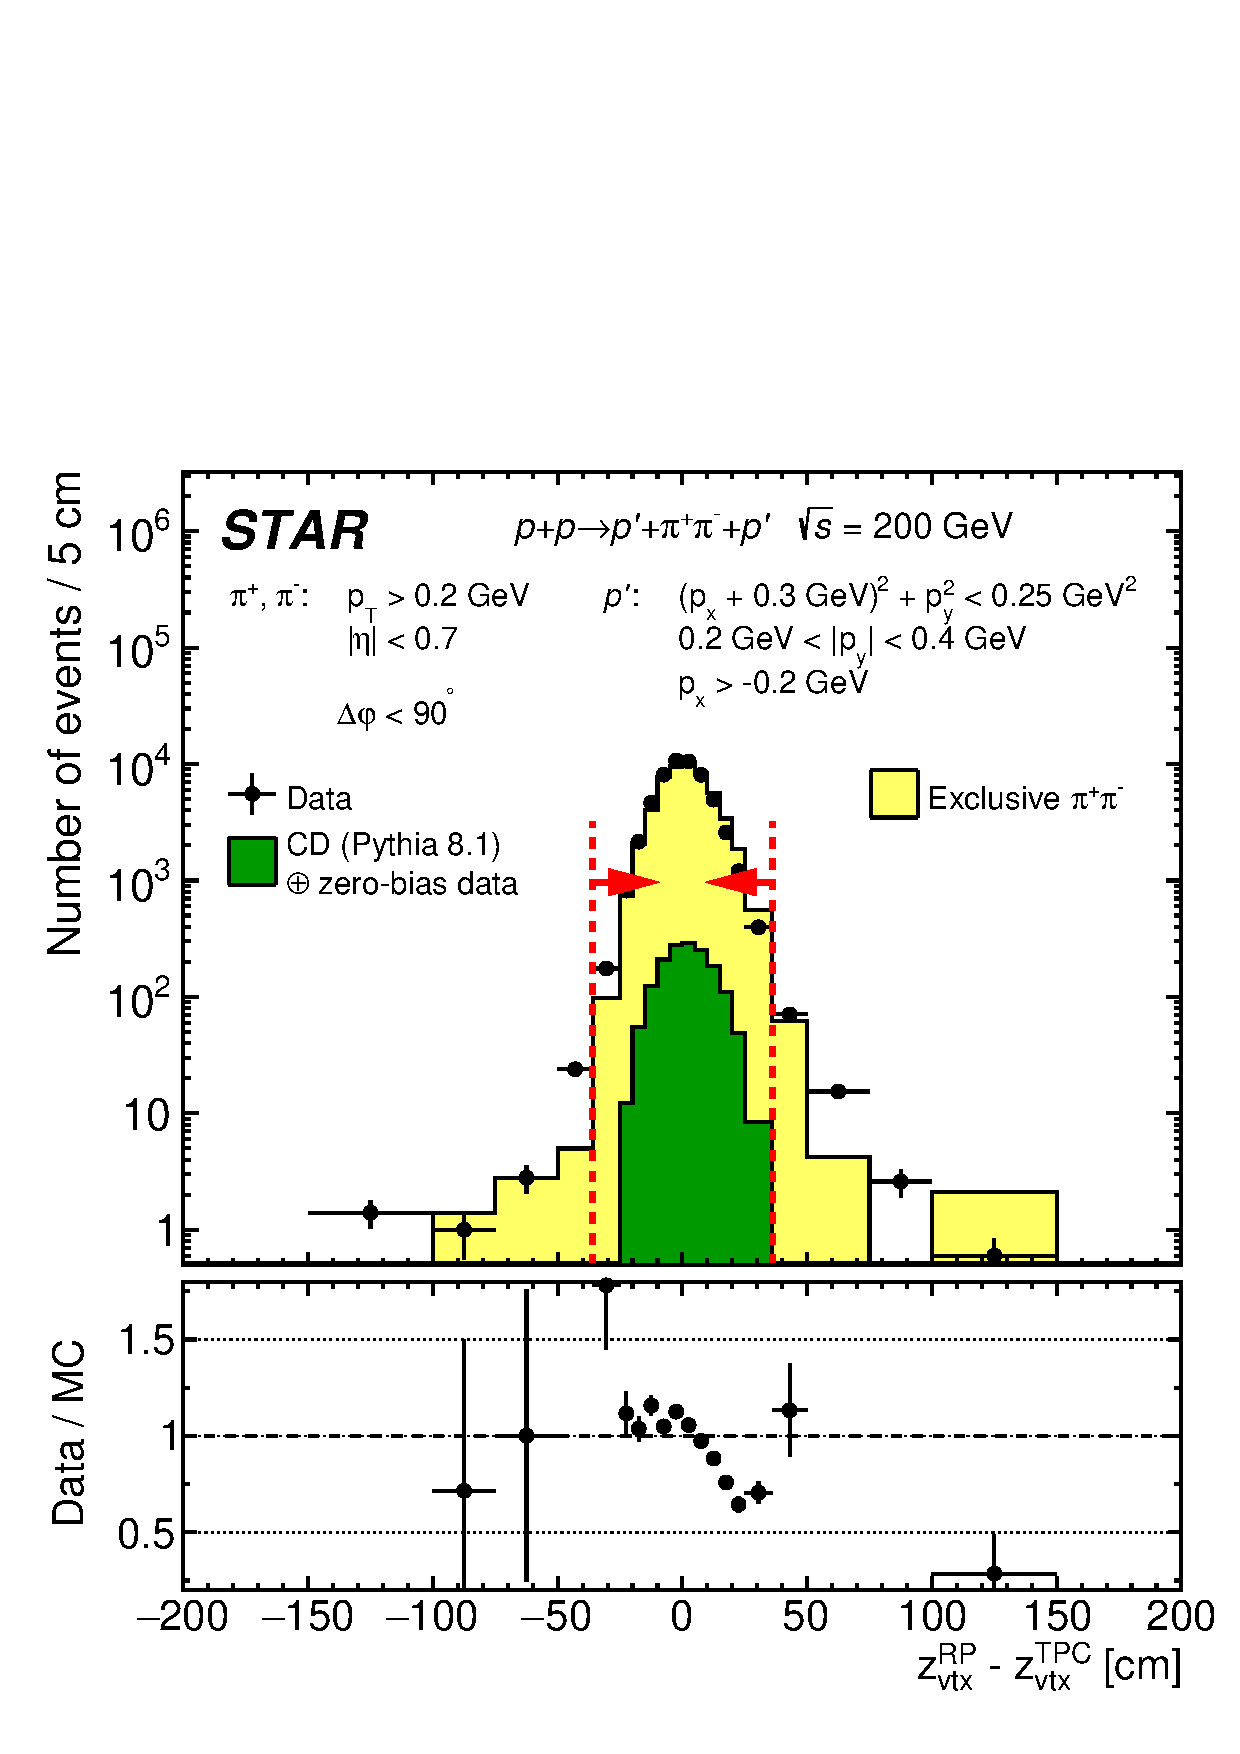
\includegraphics[width=1.05\linewidth,page=1]{graphics/backgrounds/dataVsMc/Ratio_DeltaZVtx_DeltaPhiBin_0.pdf}\vspace*{-10pt}}
  \end{subfigure}\\
  \begin{subfigure}[b]{\linewidth}\addtocounter{subfigure}{1}
                \subcaptionbox{\label{fig:Ratio_Linear_DeltaZVtx_DeltaPhiBin_0}}{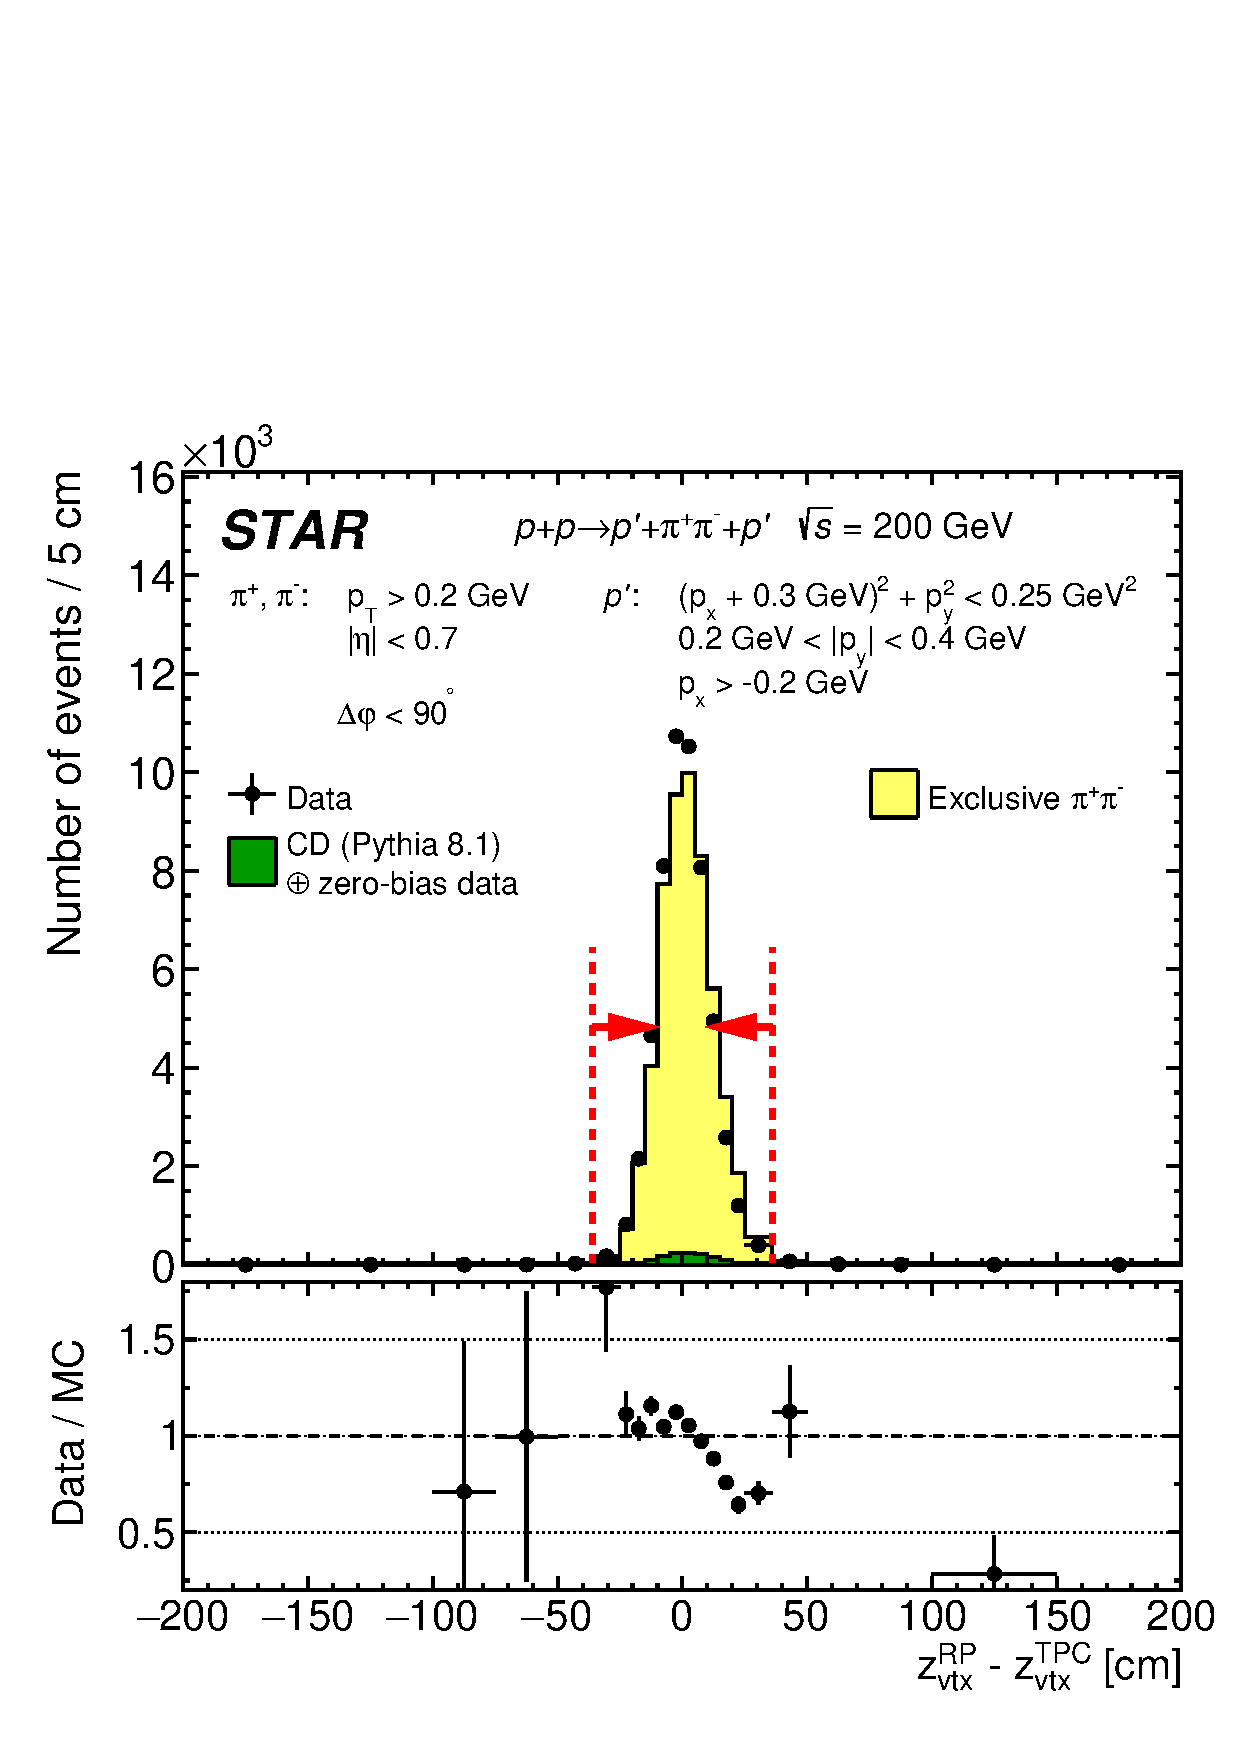
\includegraphics[width=1.05\linewidth,page=1]{graphics/backgrounds/dataVsMc/Ratio_Linear_DeltaZVtx_DeltaPhiBin_0.pdf}\vspace*{-10pt}}
  \end{subfigure}
}%
\quad\quad%
\parbox{0.4725\textwidth}{
  \centering
  \begin{subfigure}[b]{\linewidth}
                \subcaptionbox{\label{fig:Ratio_DeltaZVtx_DeltaPhiBin_1}}{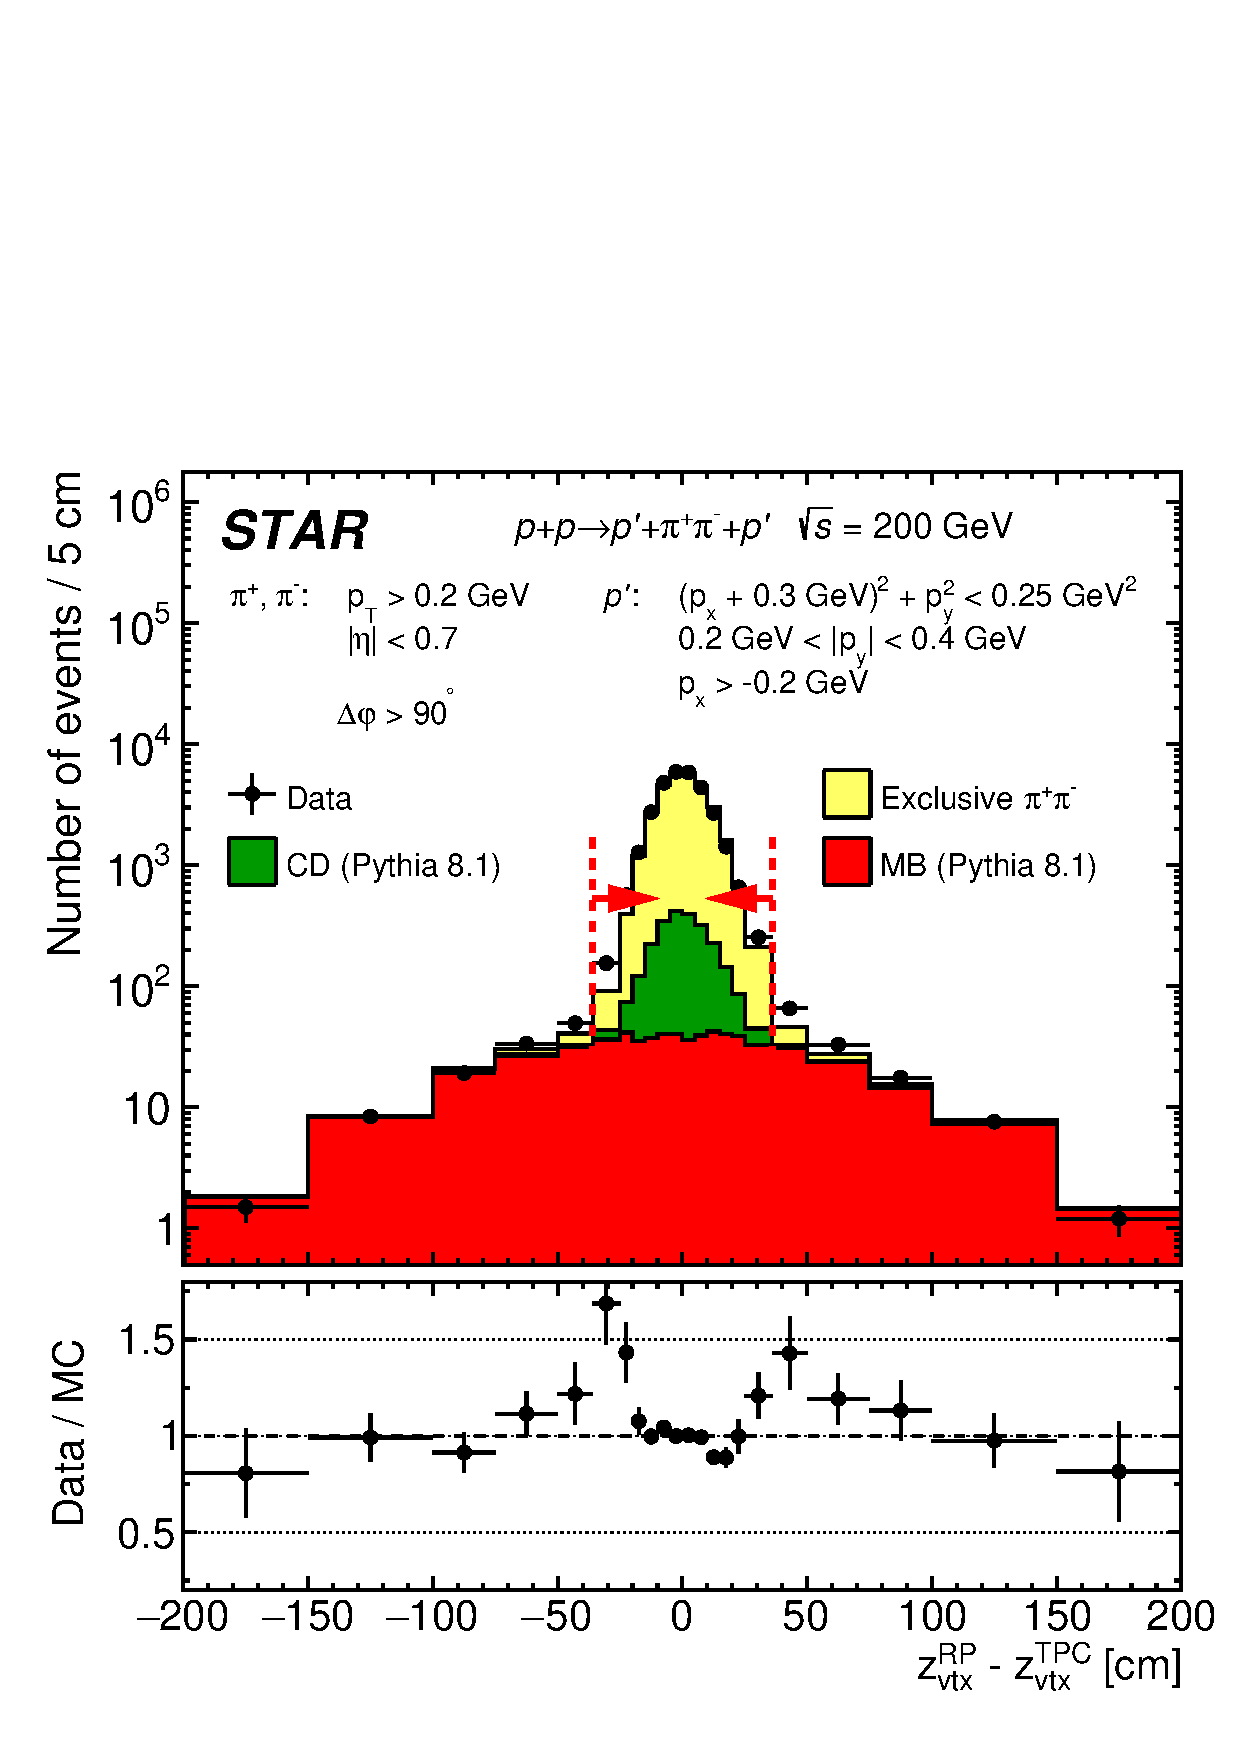
\includegraphics[width=1.05\linewidth,page=1]{graphics/backgrounds/dataVsMc/Ratio_DeltaZVtx_DeltaPhiBin_1.pdf}\vspace*{-10pt}}
  \end{subfigure}\\
  \begin{subfigure}[b]{\linewidth}\addtocounter{subfigure}{1}
                \subcaptionbox{\label{fig:Ratio_Linear_DeltaZVtx_DeltaPhiBin_1}}{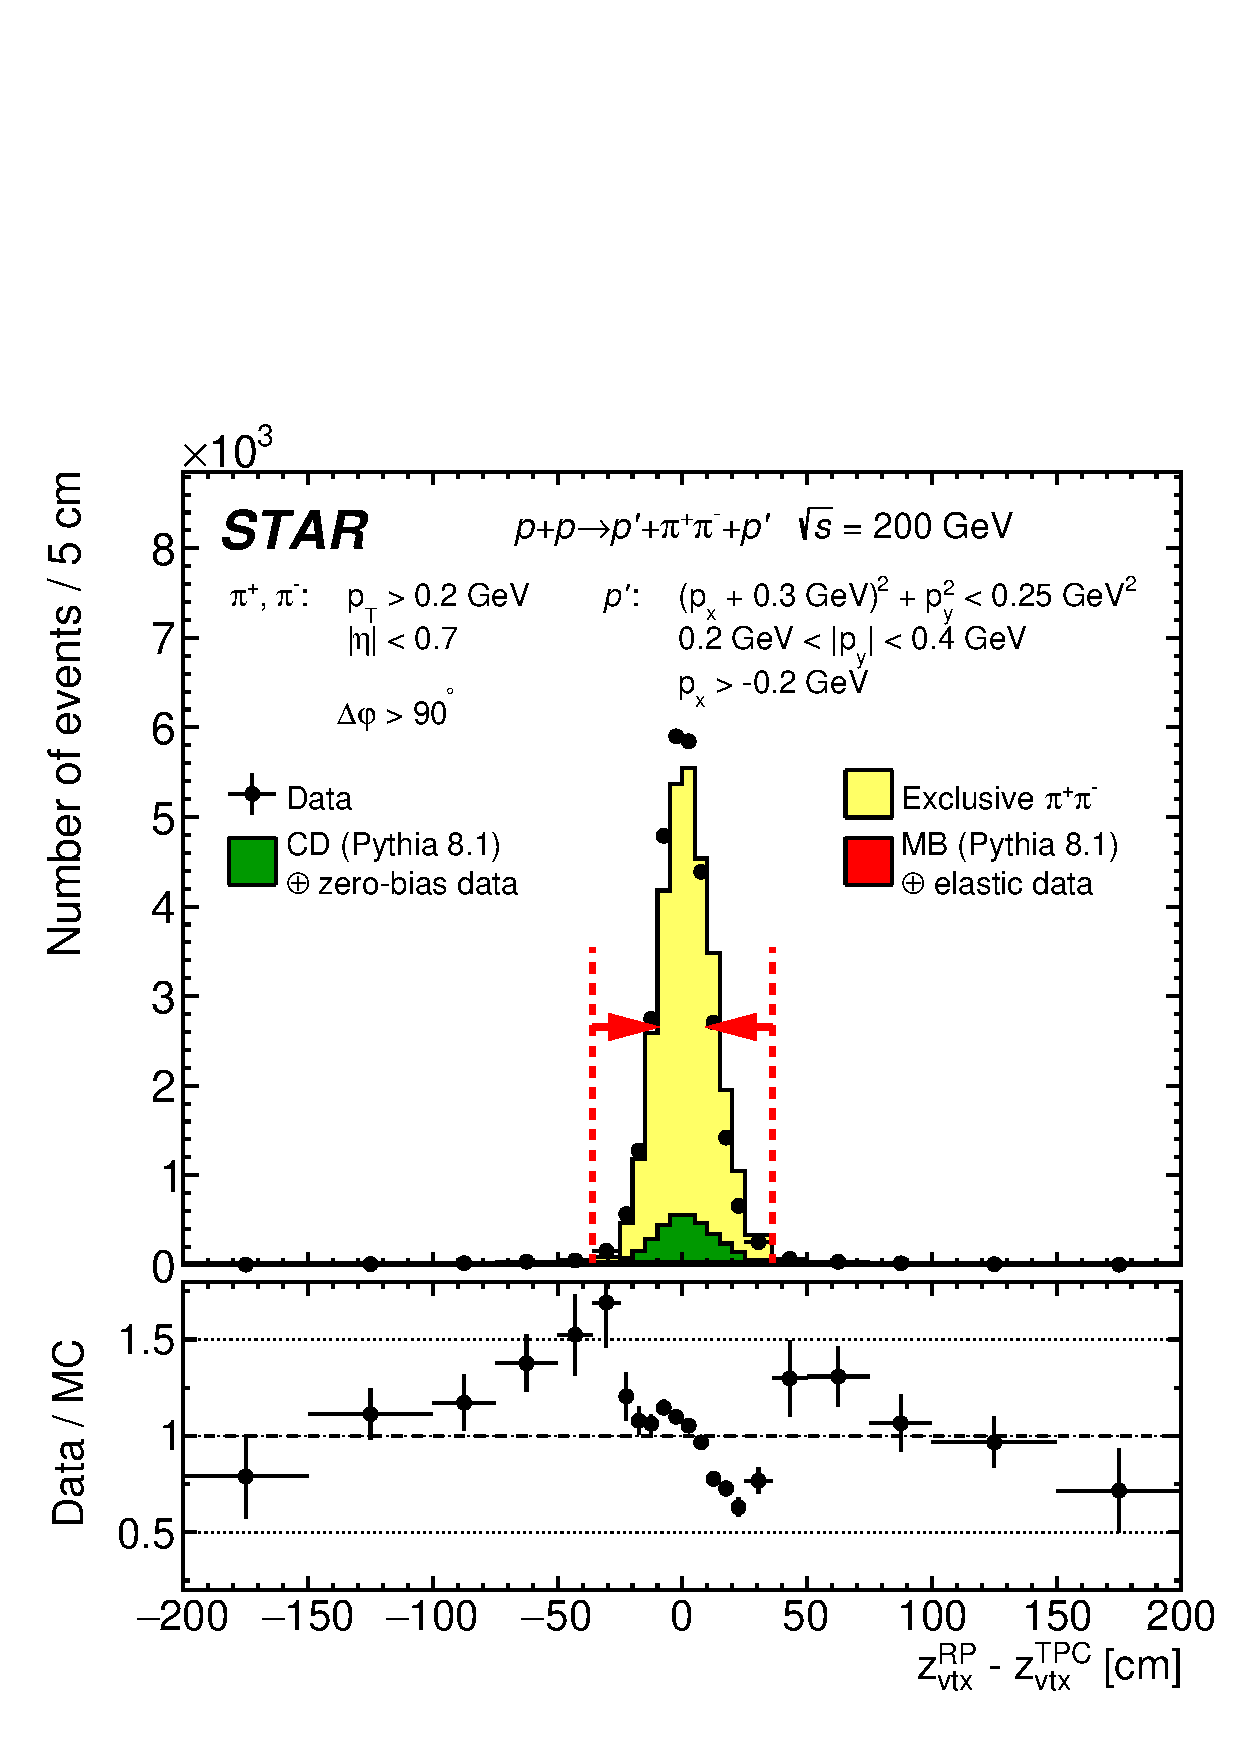
\includegraphics[width=1.05\linewidth,page=1]{graphics/backgrounds/dataVsMc/Ratio_Linear_DeltaZVtx_DeltaPhiBin_1.pdf}\vspace*{-10pt}}
  \end{subfigure} 
}\caption[Comparison of $\Delta z_{\text{vtx}}$ for CEP $\pi^{+}\pi^{-}$ events in two ranges of $\Delta\varphi$ between data and embedded MC.]{Comparison of $\Delta z_{\text{vtx}}$ for CEP $\pi^{+}\pi^{-}$ events in two ranges of $\Delta\varphi$ (left: $\Delta\varphi<90^{\circ}$, right: $\Delta\varphi>90^{\circ}$) between data and embedded MC after full selection (except cut on presented quantity). Plots in top and bottom row differ only in the $y$-axis (top: logarithmic, bottom: linear). Data are represented by black points, while stacked MC predictions are drawn as histograms of different colors. Histogram from each MC process has been normalized according to prescription in the text. Vertical error bars represent statistical uncertainties, horizontal bars represent bin sizes.}\label{fig:Ratio_DeltaZVtx_DeltaPhiBins}%
\end{figure}
%--------------------------- 


\begin{figure}[h]
\centering
\parbox{0.4725\textwidth}{
  \centering
  \begin{subfigure}[b]{\linewidth}
                \subcaptionbox{\label{fig:Ratio_DZVtx}}{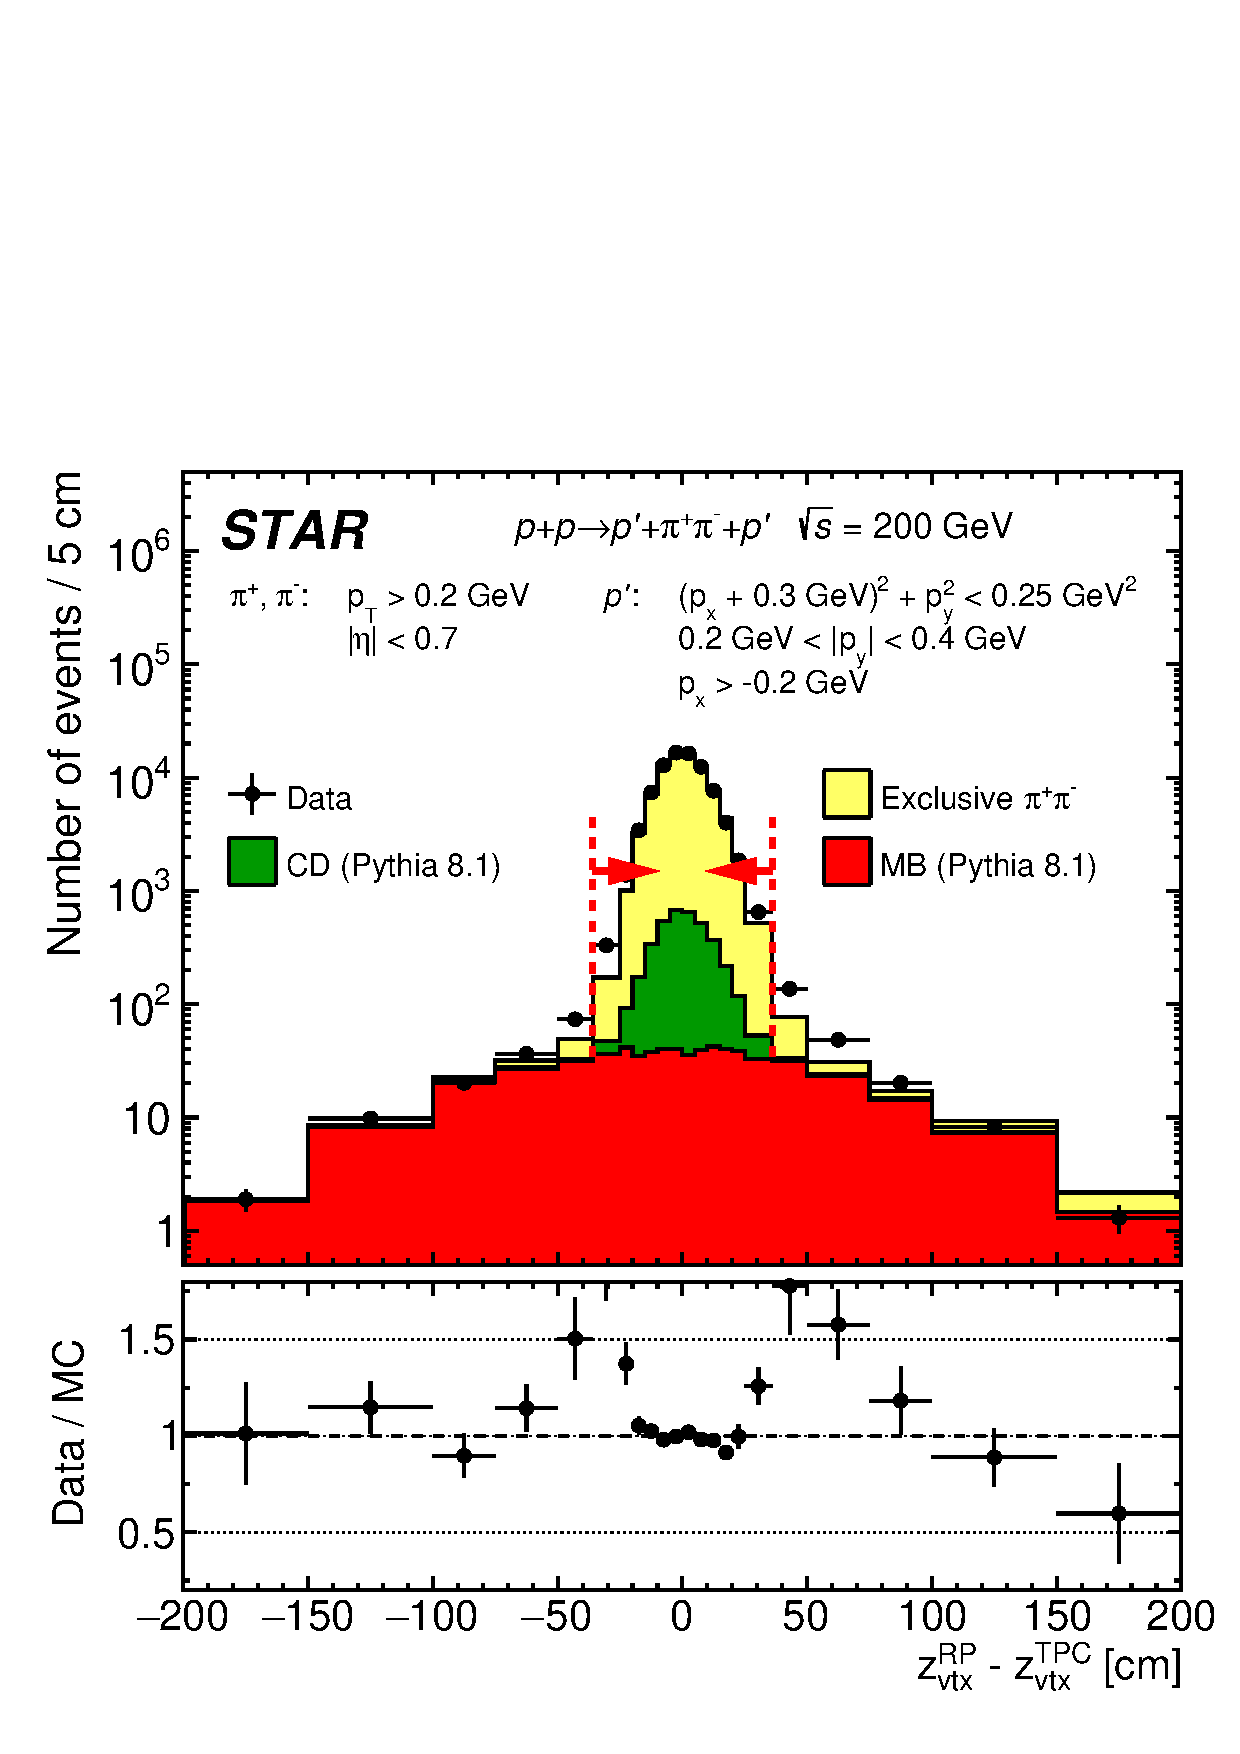
\includegraphics[width=1.05\linewidth,page=1]{graphics/backgrounds/dataVsMc/Ratio_DeltaZVtx.pdf}}
  \end{subfigure}
}%
\quad\quad%
\parbox{0.4725\textwidth}{
  \centering
  \begin{subfigure}[b]{\linewidth}
                \subcaptionbox{\label{fig:Ratio_Linear_DeltaZVtx}}{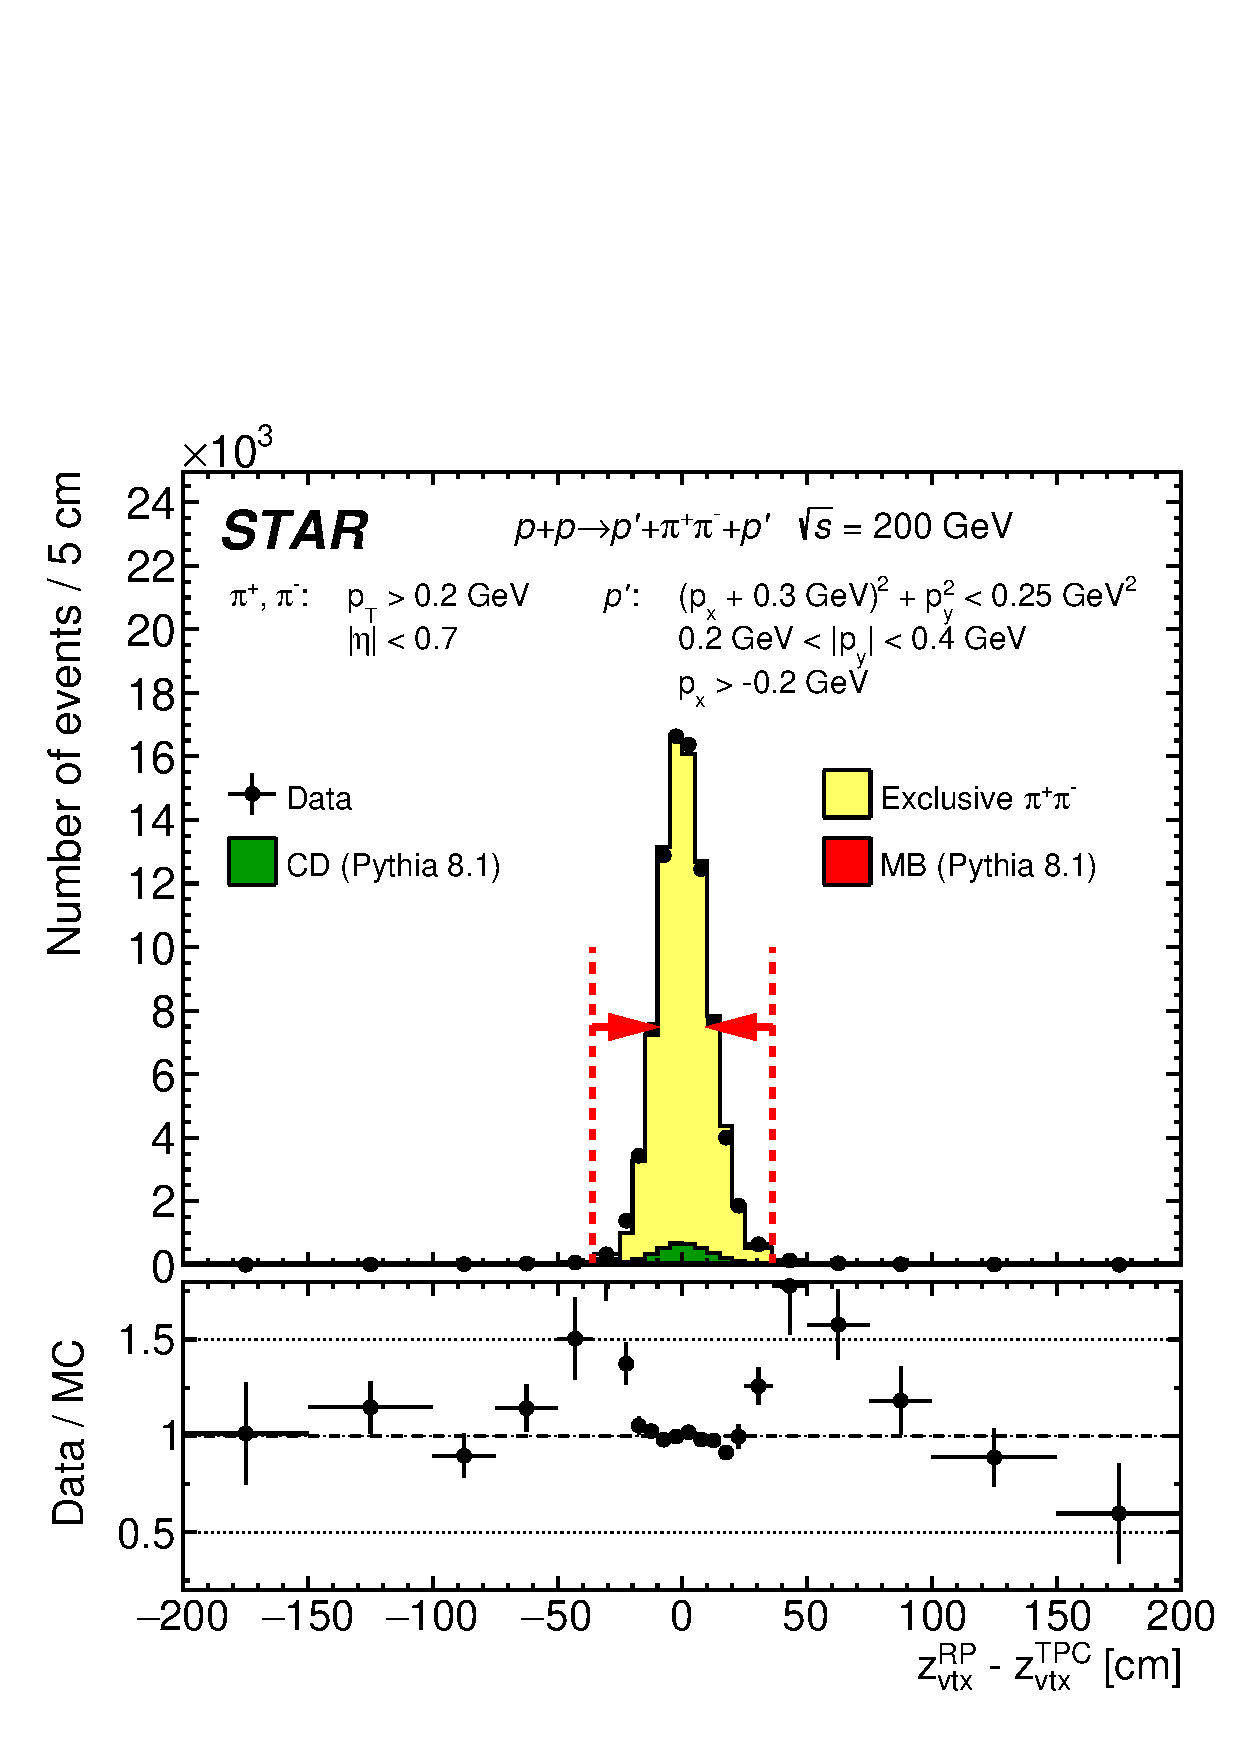
\includegraphics[width=1.05\linewidth,page=1]{graphics/backgrounds/dataVsMc/Ratio_Linear_DeltaZVtx.pdf}}
  \end{subfigure}
}\caption[Comparison of $\Delta z_{\text{vtx}}$ for CEP $\pi^{+}\pi^{-}$ events between data and embedded MC.]{Comparison of $\Delta z_{\text{vtx}}$ for CEP $\pi^{+}\pi^{-}$ events between data and embedded MC after full selection (except cut on presented quantity). Left and right plot differ only in the $y$-axis (left: logarithmic, right: linear). Data are represented by black points, while stacked MC predictions are drawn as histograms of different colors. Histogram from each MC process has been normalized according to prescription in the text. Vertical error bars represent statistical uncertainties, horizontal bars represent bin sizes.}\label{fig:Ratio_DeltaZVtx}%
\end{figure}
%---------------------------







%---------------------------
\begin{figure}[ht!]
\centering%
\parbox{0.4725\textwidth}{%
  \centering%
  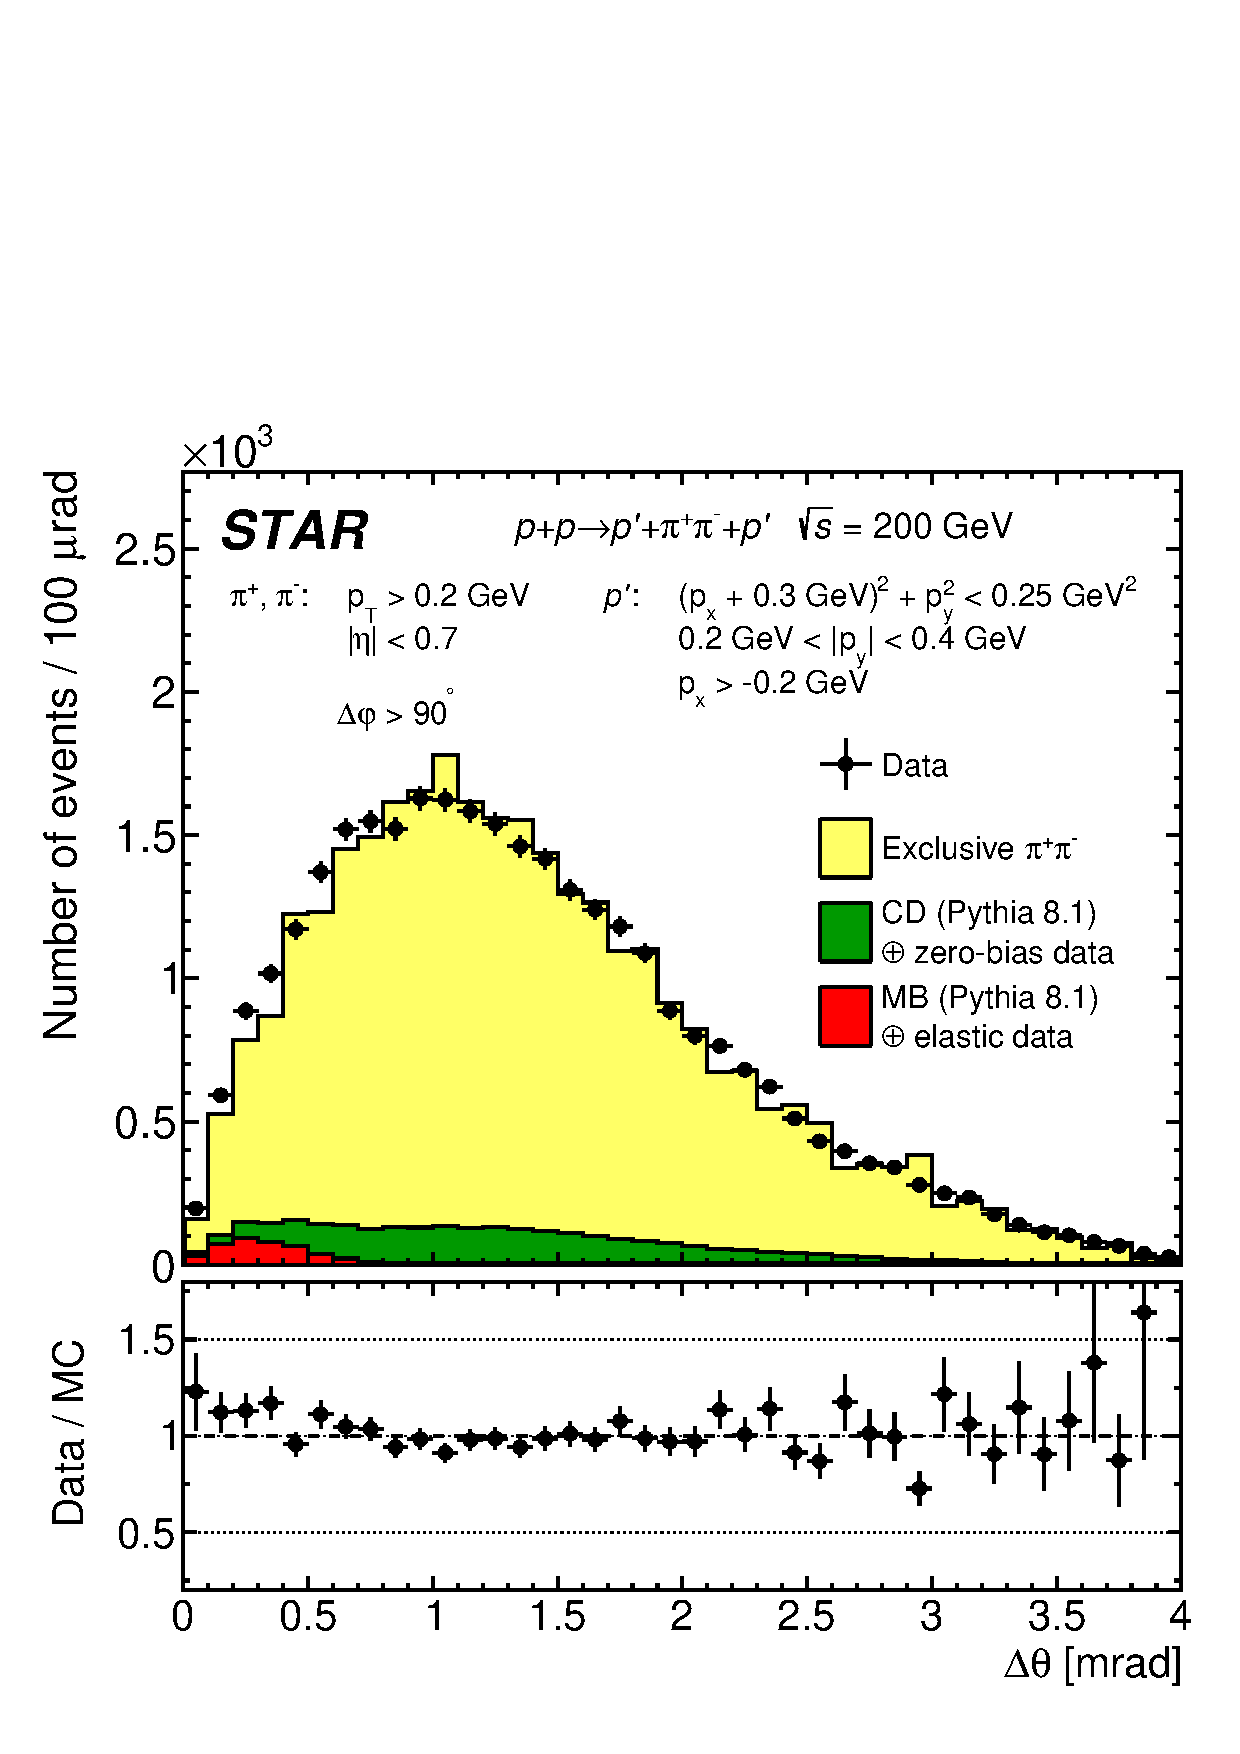
\includegraphics[width=\linewidth]{graphics/backgrounds/dataVsMc/Ratio_Collinearity.pdf}
}%
\quad%
\parbox{0.4725\textwidth}{%
    \caption[Comparison of collinearity $\Delta\theta$ for CEP $\pi^{+}\pi^{-}$ events with $\Delta\varphi>90^{\circ}$, between data and embedded MC.]{Comparison of coliinearity $\Delta\theta$ for CEP $\pi^{+}\pi^{-}$ events with $\Delta\varphi>90^{\circ}$ between data and embedded MC after full selection. Data are represented by black points, while stacked MC predictions are drawn as histograms of different colors. Histogram from each MC process has been normalized according to prescription in the text. Vertical error bars represent statistical uncertainties, horizontal bars represent bin sizes.}\label{fig:Ratio_Collinearity}%  
}
\end{figure}
%---------------------------






\begin{figure}[h]
\centering
\parbox{0.4725\textwidth}{
  \centering
  \begin{subfigure}[b]{\linewidth}
                \subcaptionbox{\label{fig:Ratio_MissingPt_OppositeAndSameSign_DeltaPhiBin_0}}{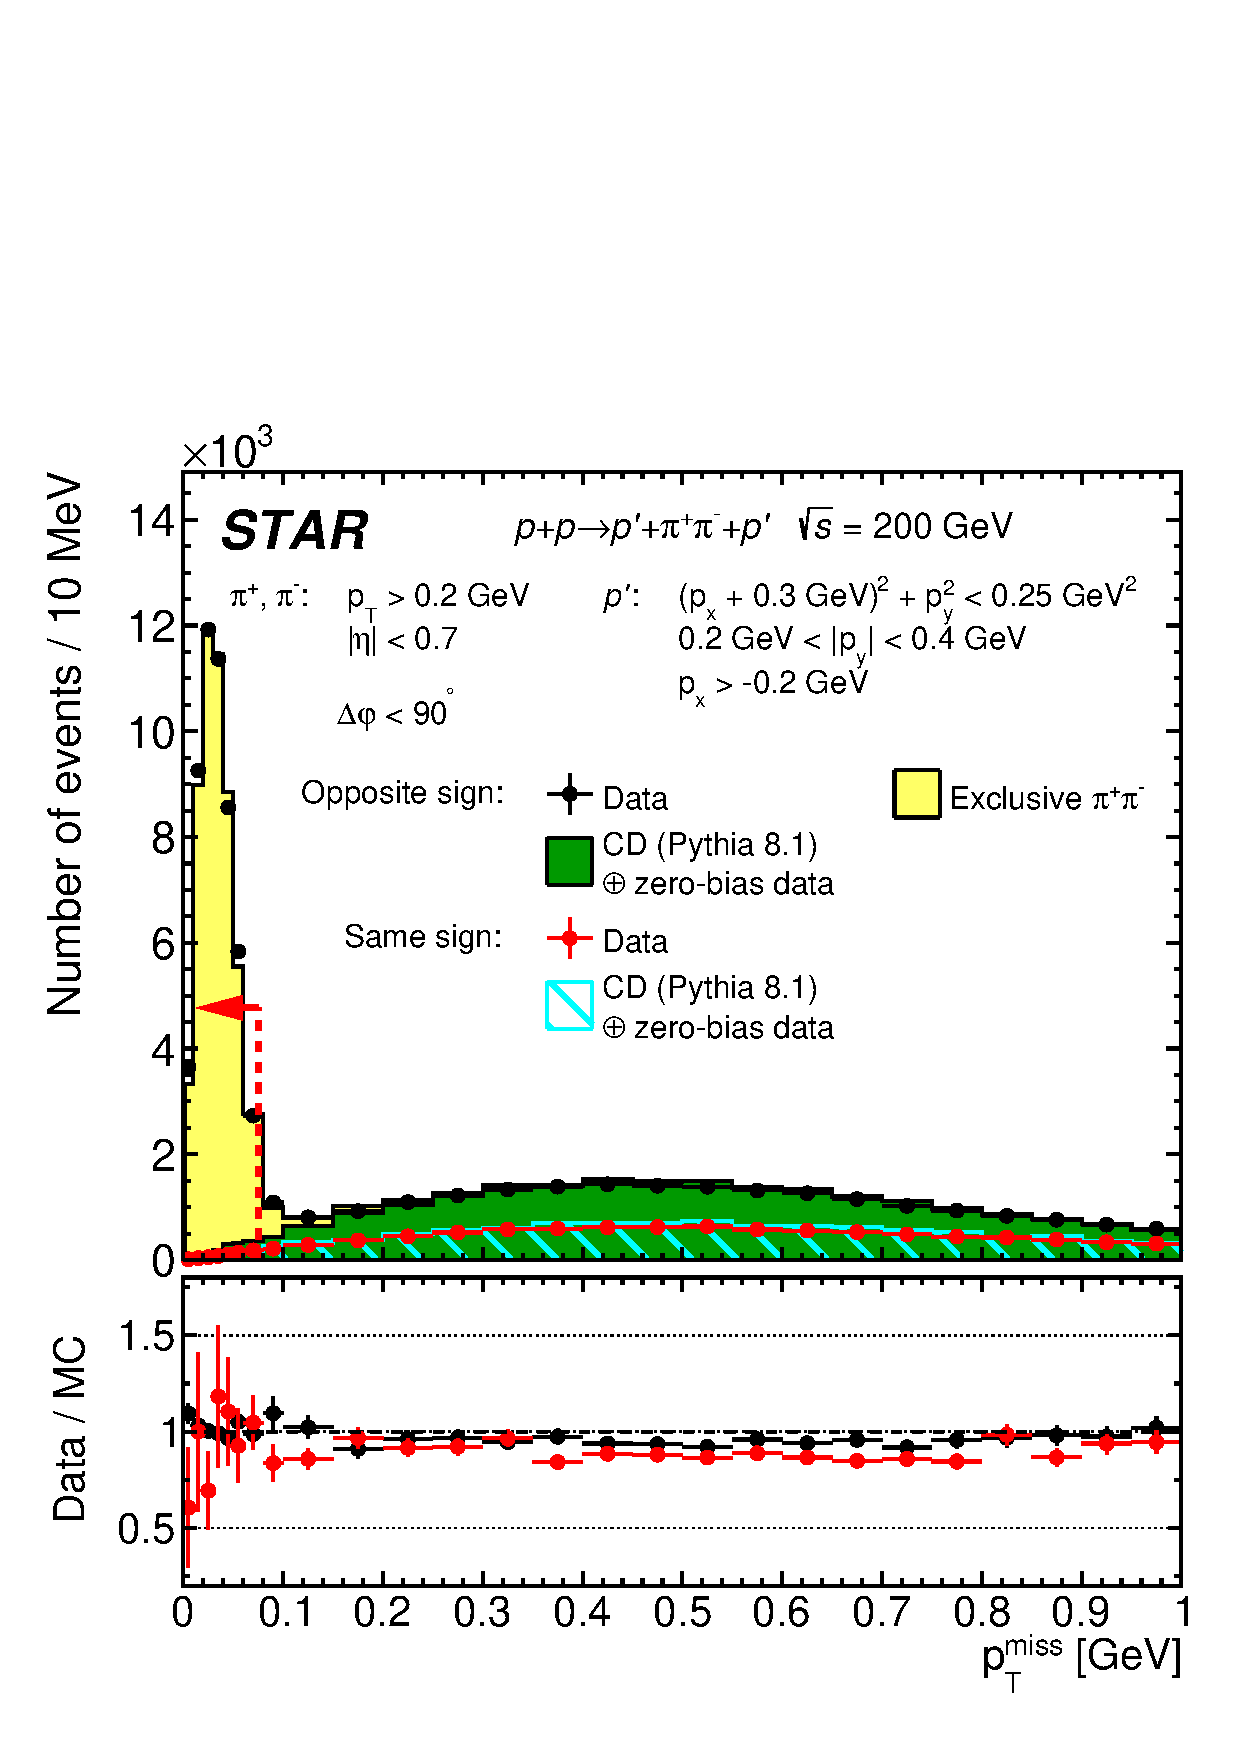
\includegraphics[width=1.05\linewidth,page=1]{graphics/backgrounds/dataVsMc/Ratio_MissingPt_OppositeAndSameSign_DeltaPhiBin_0.pdf}}
  \end{subfigure}\\
  \begin{subfigure}[b]{\linewidth}\addtocounter{subfigure}{1}
                \subcaptionbox{\label{fig:Ratio_LogY_MissingPt_OppositeAndSameSign_DeltaPhiBin_0}}{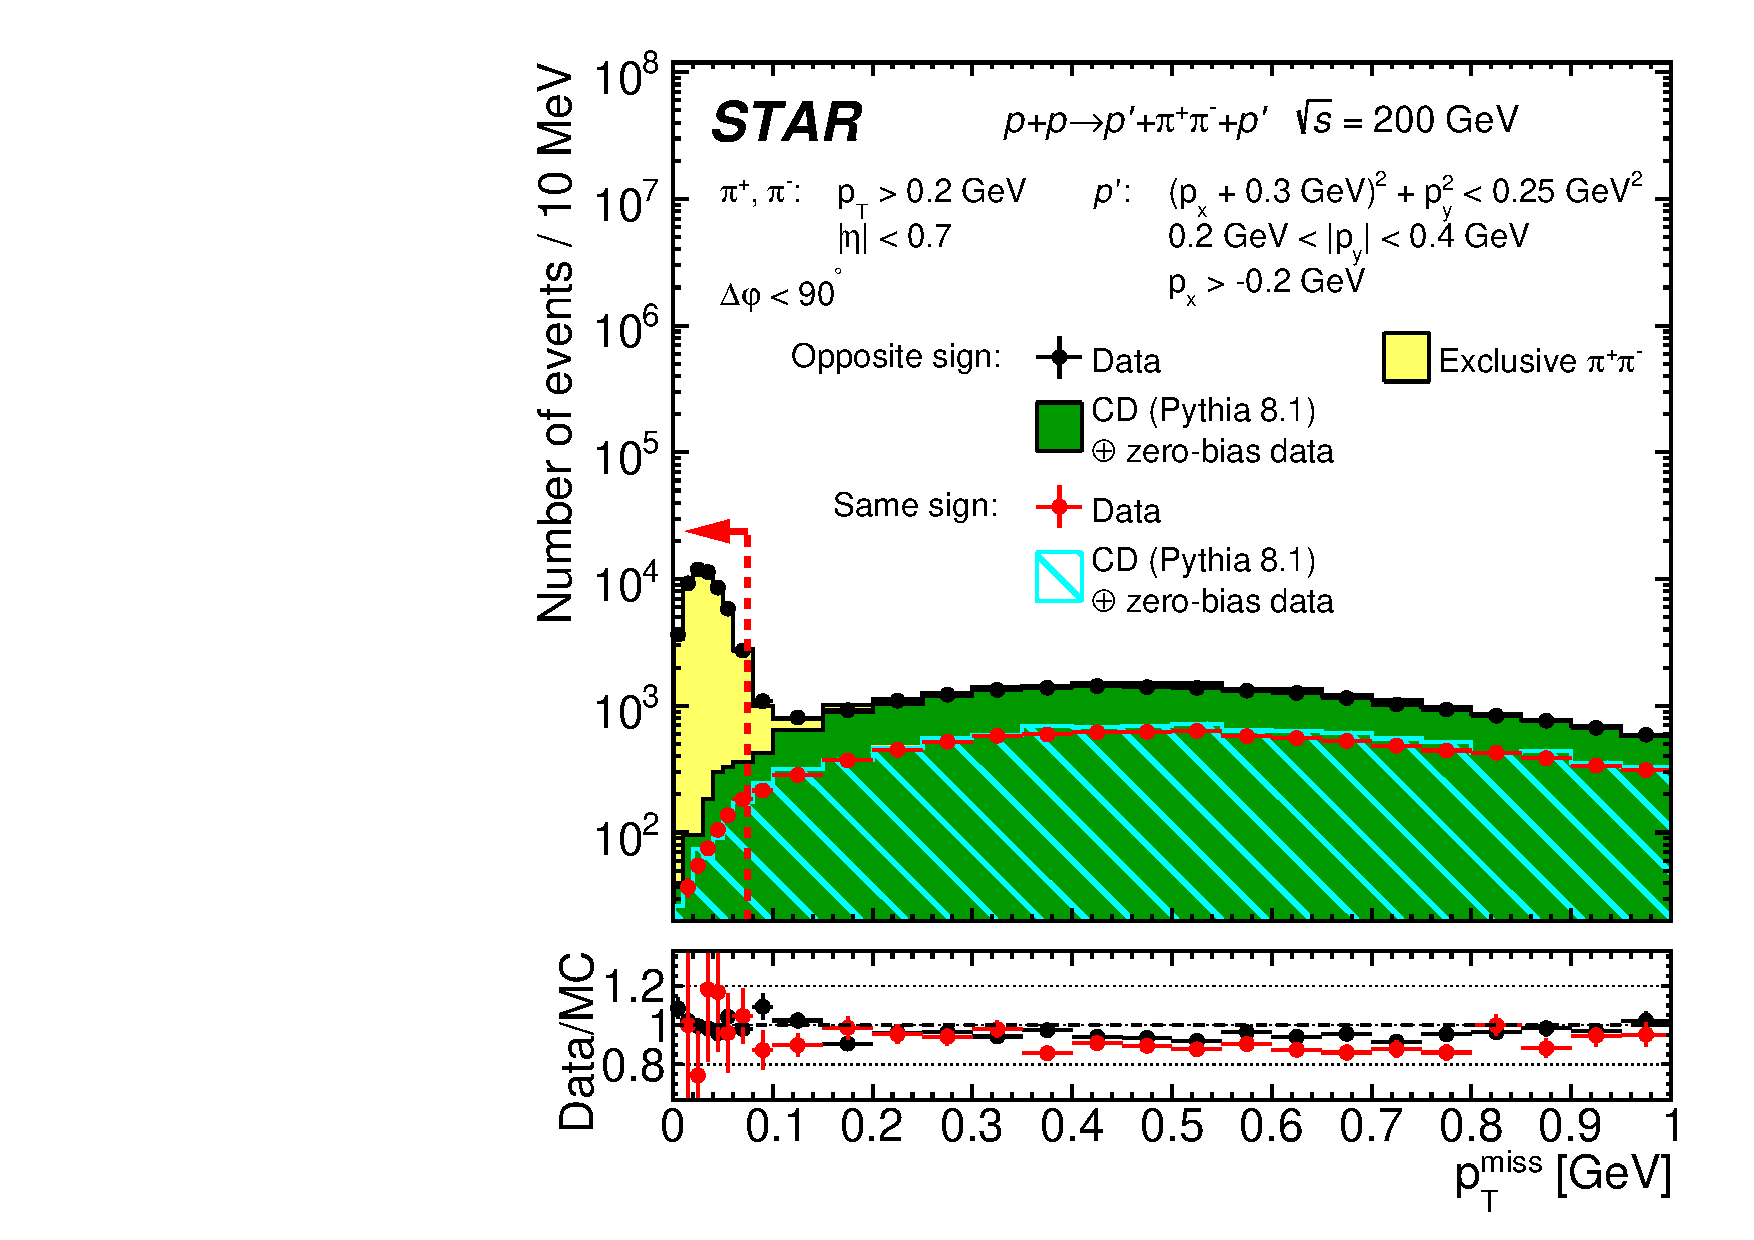
\includegraphics[width=1.05\linewidth,page=1]{graphics/backgrounds/dataVsMc/Ratio_LogY_MissingPt_OppositeAndSameSign_DeltaPhiBin_0.pdf}}
  \end{subfigure} 
}%
\quad\quad%
\parbox{0.4725\textwidth}{
  \centering
  \begin{subfigure}[b]{\linewidth}
                \subcaptionbox{\label{fig:Ratio_MissingPt_OppositeAndSameSign_DeltaPhiBin_1}}{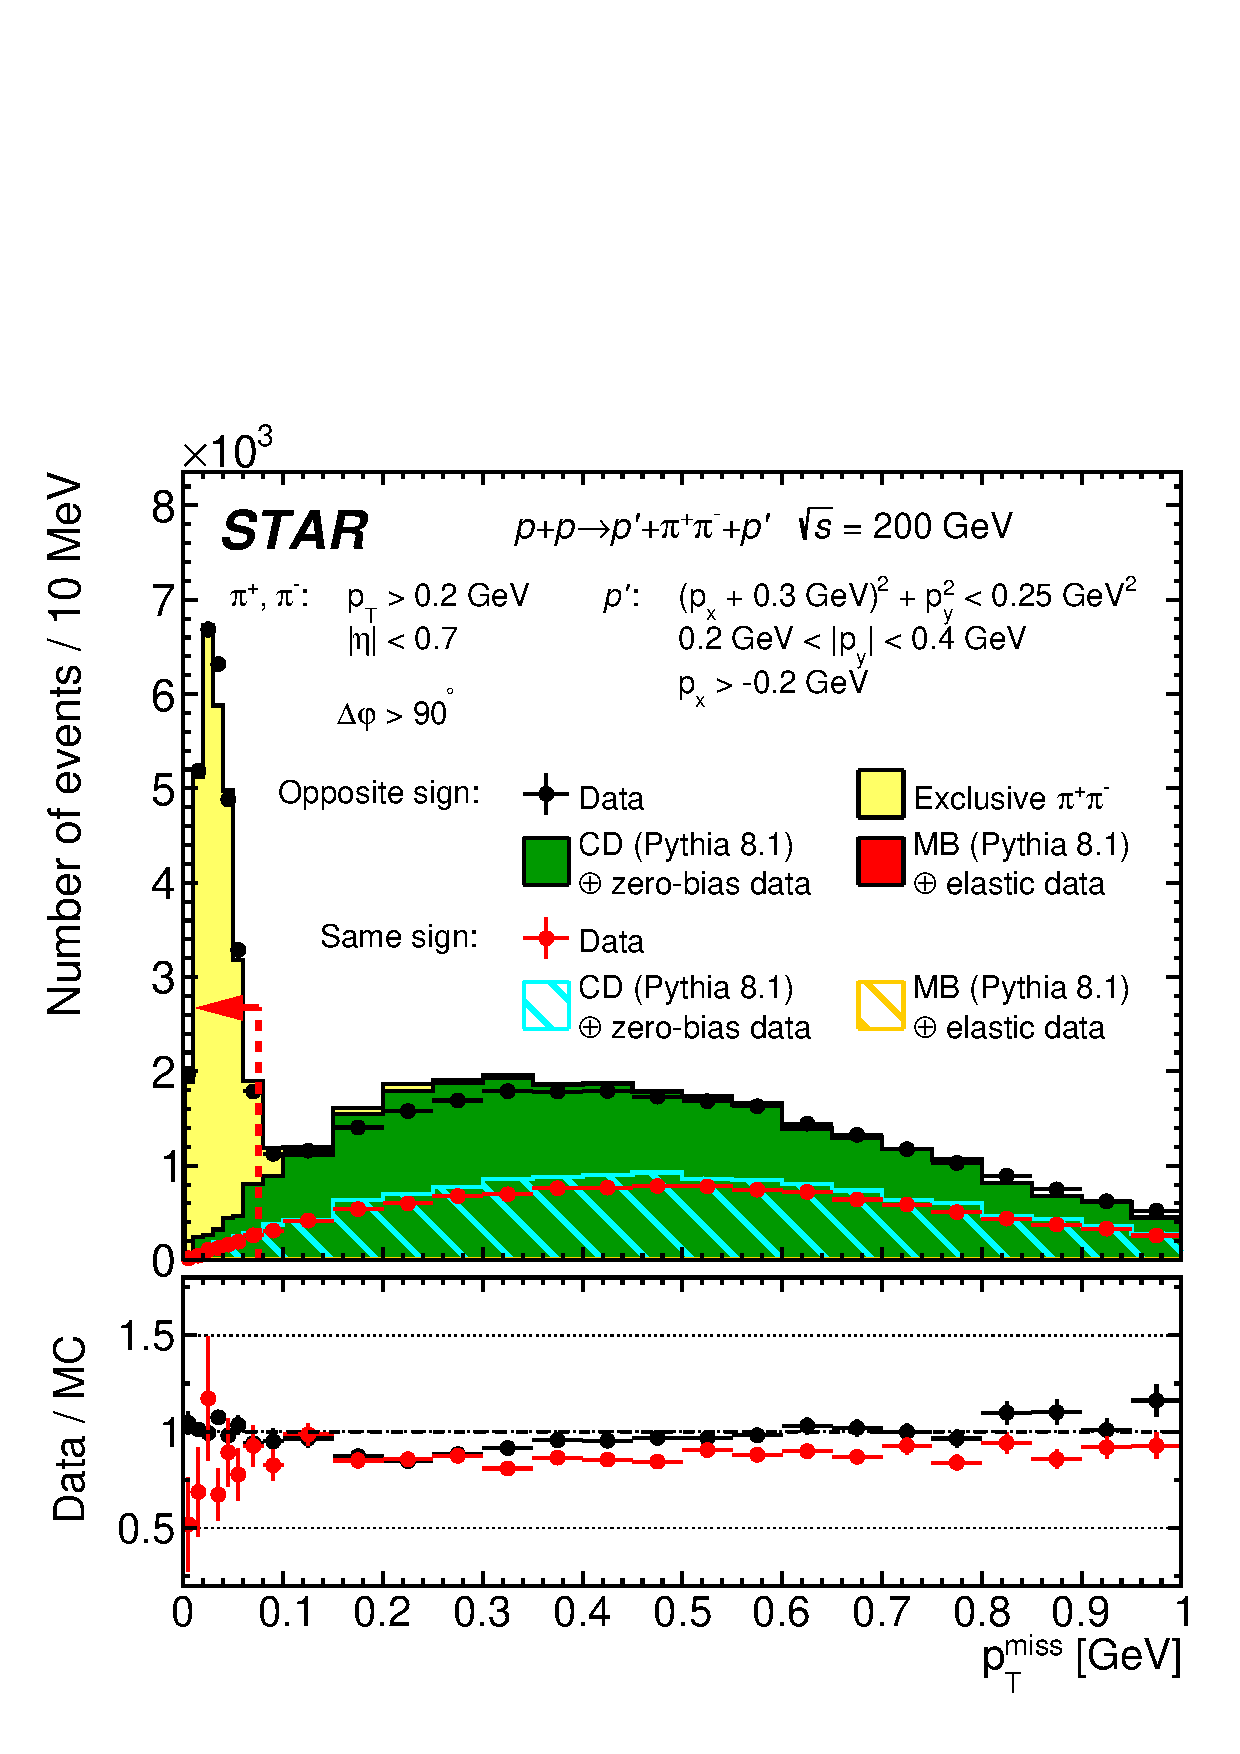
\includegraphics[width=1.05\linewidth,page=1]{graphics/backgrounds/dataVsMc/Ratio_MissingPt_OppositeAndSameSign_DeltaPhiBin_1.pdf}}
  \end{subfigure}\\
  \begin{subfigure}[b]{\linewidth}\addtocounter{subfigure}{1}
                \subcaptionbox{\label{fig:Ratio_LogY_MissingPt_OppositeAndSameSign_DeltaPhiBin_1}}{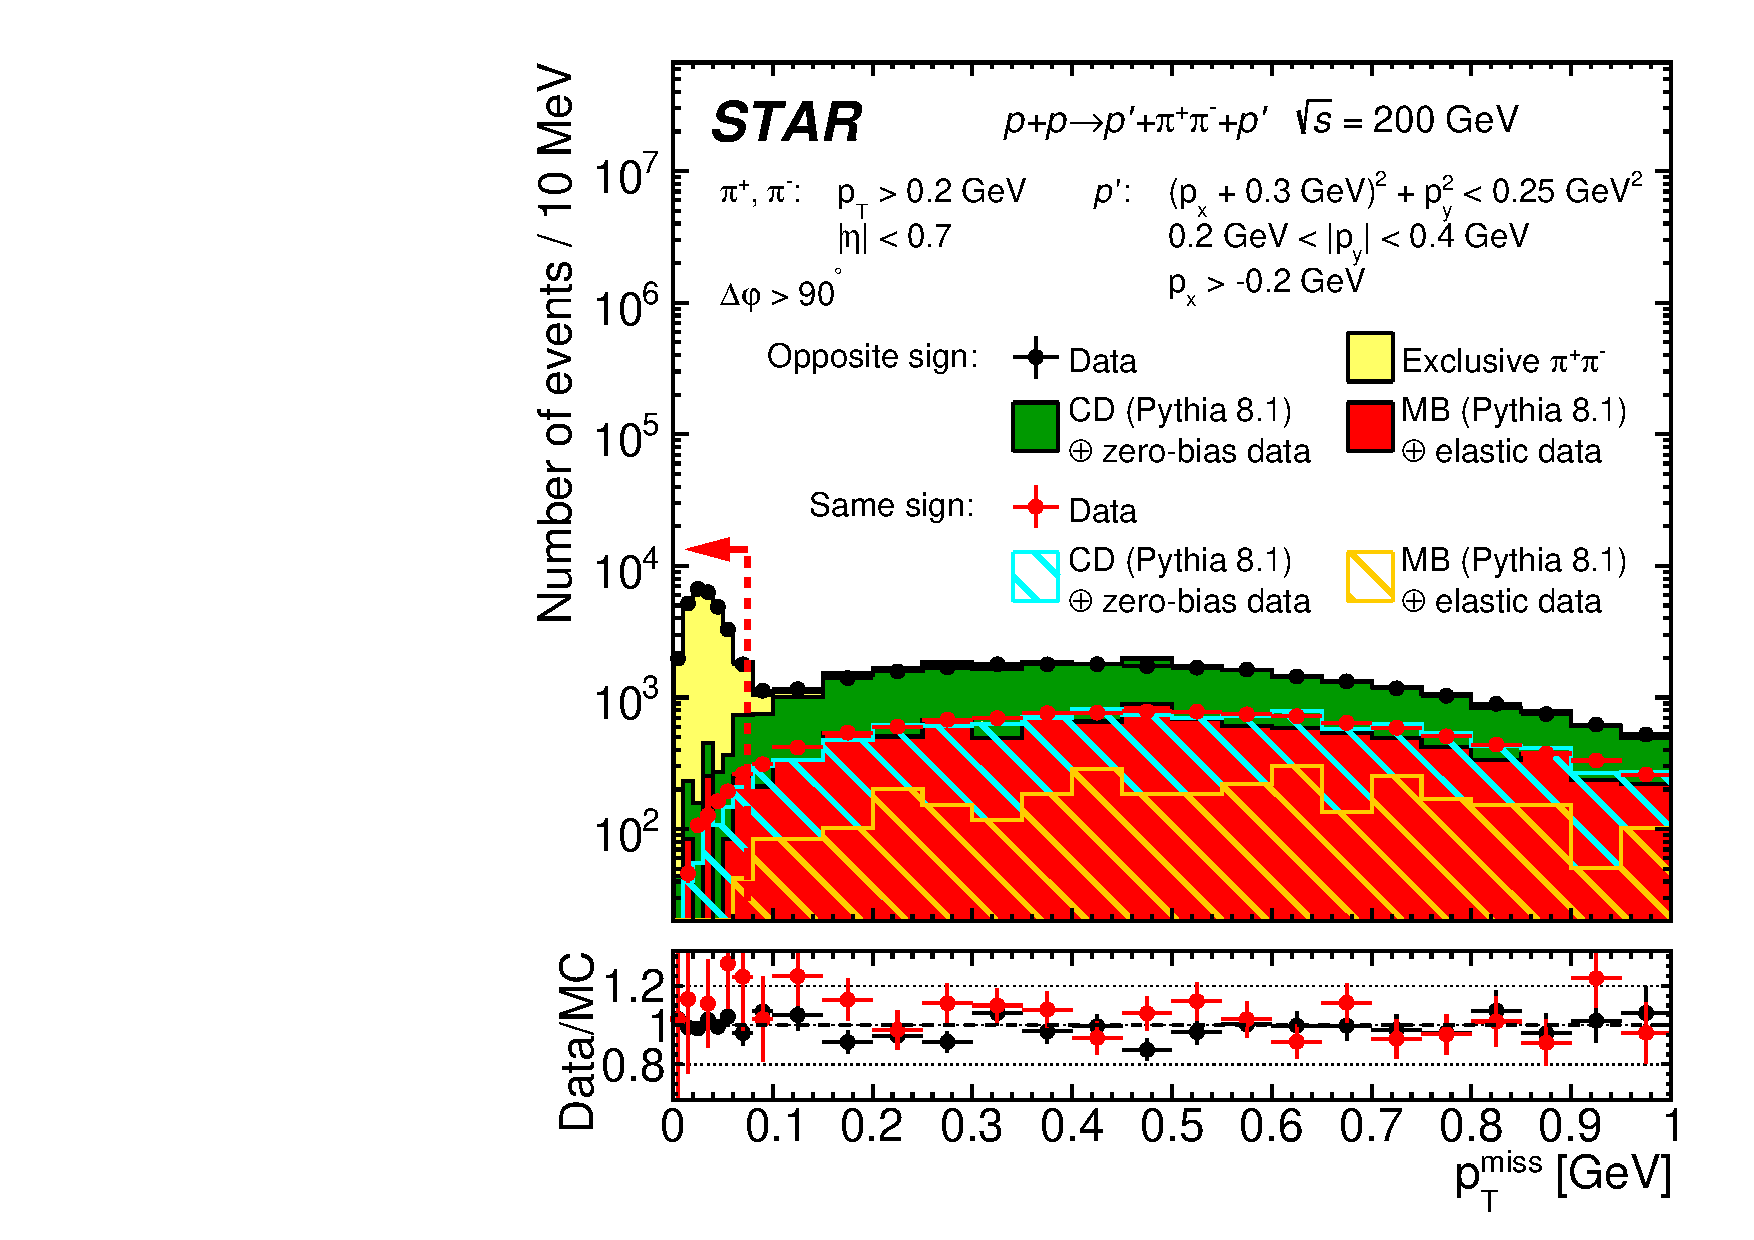
\includegraphics[width=1.05\linewidth,page=1]{graphics/backgrounds/dataVsMc/Ratio_LogY_MissingPt_OppositeAndSameSign_DeltaPhiBin_1.pdf}}
  \end{subfigure} 
}\caption[Comparison of $p_{T}^{\text{miss}}$ for CEP $\pi^{+}\pi^{-}$ events in two ranges of $\Delta\varphi$ between data and embedded MC.]{Comparison of $p_{T}^{\text{miss}}$ for CEP $\pi^{+}\pi^{-}$ events in two ranges of $\Delta\varphi$ (left: $\Delta\varphi<90^{\circ}$, right: $\Delta\varphi>90^{\circ}$) between data and embedded MC after full selection (except cut on presented quantity). Plots in top and bottom row differ only in the $y$-axis (top: linear, bottom: logarithmic). In addition to signal channel (opposite-sign particles) also control background channel (same-sign particles) is contained in the plots. Data are represented by black (opposite-sign) or red (same-sign) points, while stacked MC predictions are drawn as filled (opposite-sign) or hatched (same-sign) histograms of different colors. Histogram from each MC process has been normalized according to prescription in the text. Vertical error bars represent statistical uncertainties, horizontal bars represent bin sizes.}\label{fig:Ratio_MissingPt_OppositeAndSameSign_DeltaPhiBins}%
\end{figure}
%--------------------------- 



\begin{figure}[h]
\centering
\parbox{0.4725\textwidth}{
  \centering
  \begin{subfigure}[b]{\linewidth}
                \subcaptionbox{\label{fig:Ratio_MissingPt_OppositeAndSameSign}}{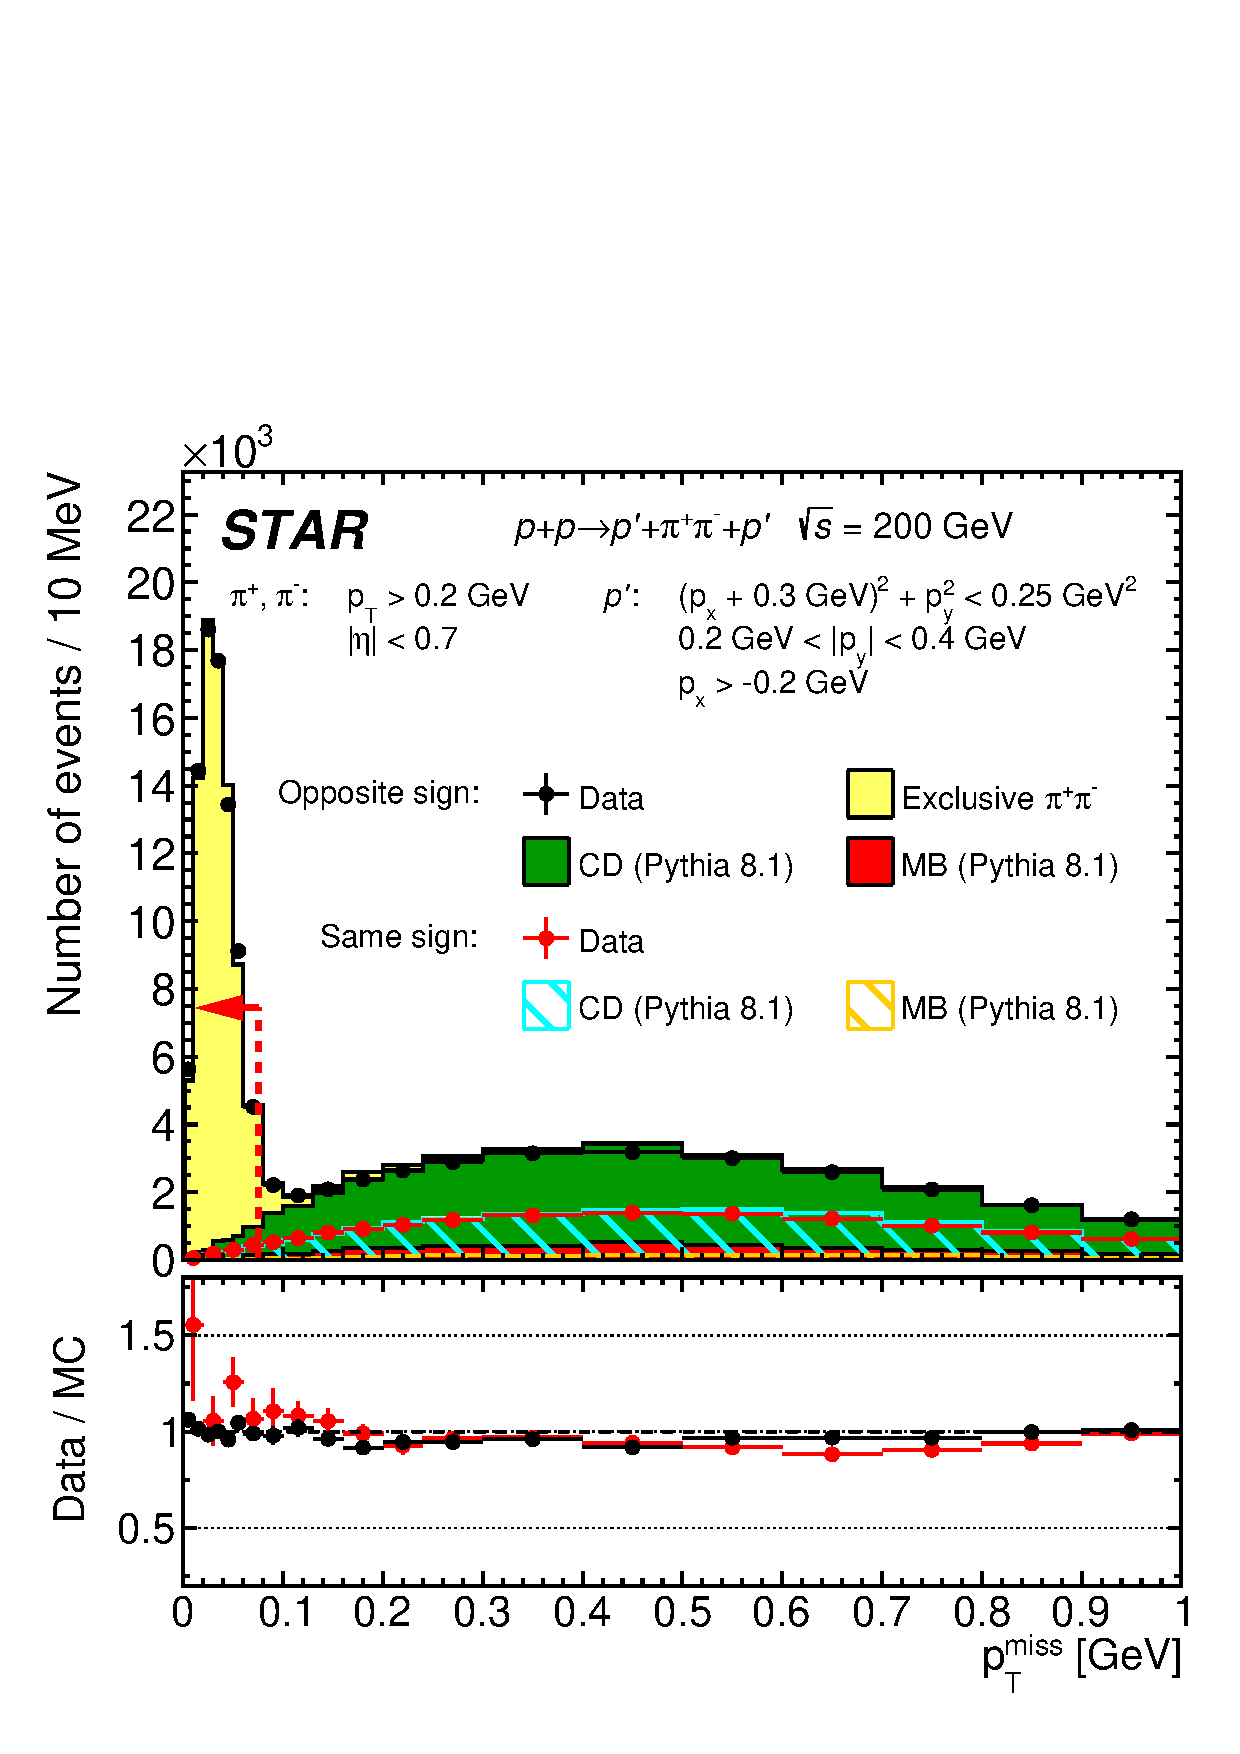
\includegraphics[width=1.05\linewidth,page=1]{graphics/backgrounds/dataVsMc/Ratio_MissingPt_OppositeAndSameSign.pdf}}
  \end{subfigure}\\
  \begin{subfigure}[b]{\linewidth}\addtocounter{subfigure}{1}
                \subcaptionbox{\label{fig:Ratio_MissingPt_OppositeAndSameSign_NeutralsNotSubtracted}}{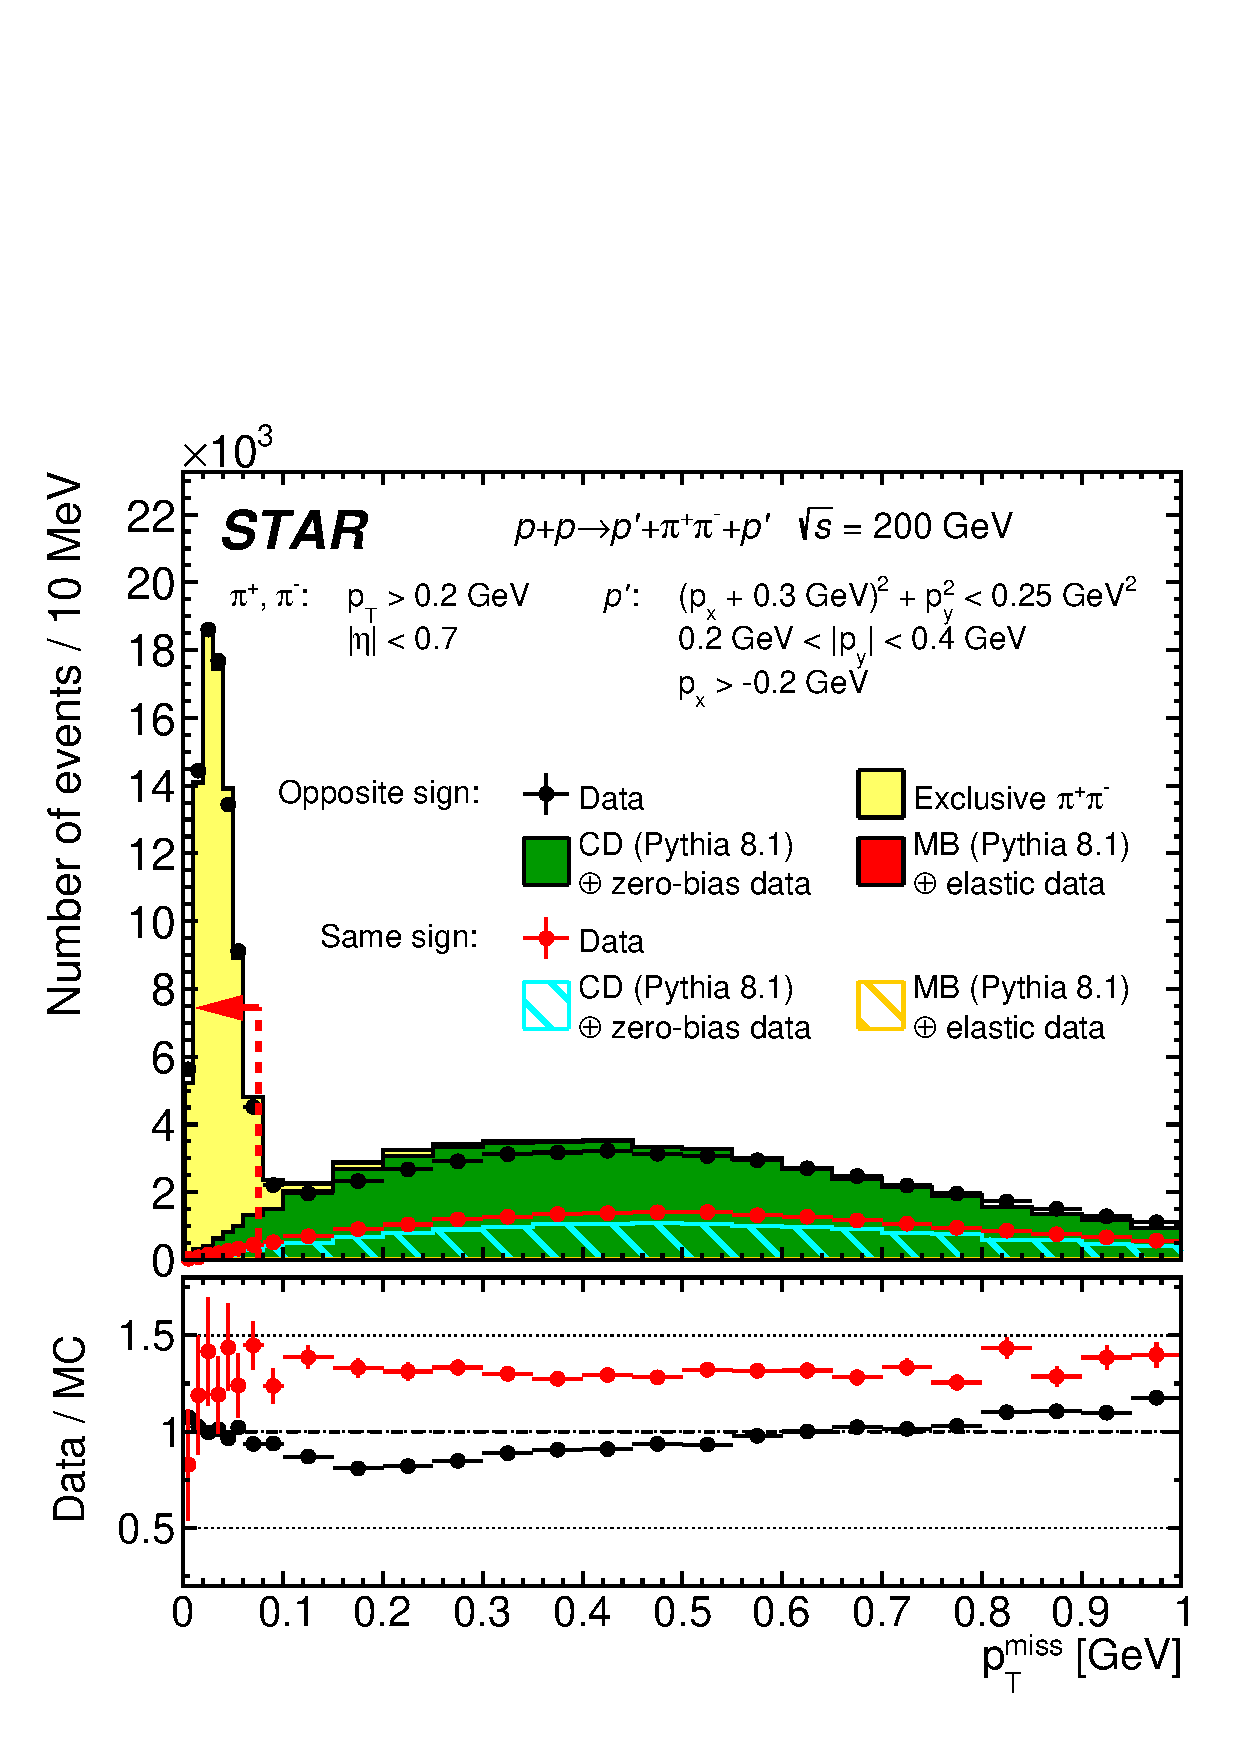
\includegraphics[width=1.05\linewidth,page=1]{graphics/backgrounds/dataVsMc/Ratio_MissingPt_OppositeAndSameSign_NeutralsNotSubtracted.pdf}}
  \end{subfigure} 
}%
\quad\quad%
\parbox{0.4725\textwidth}{
  \centering
  \begin{subfigure}[b]{\linewidth}\vspace*{-45pt}
                \subcaptionbox{\label{fig:Ratio_LogY_MissingPt_OppositeAndSameSign}}{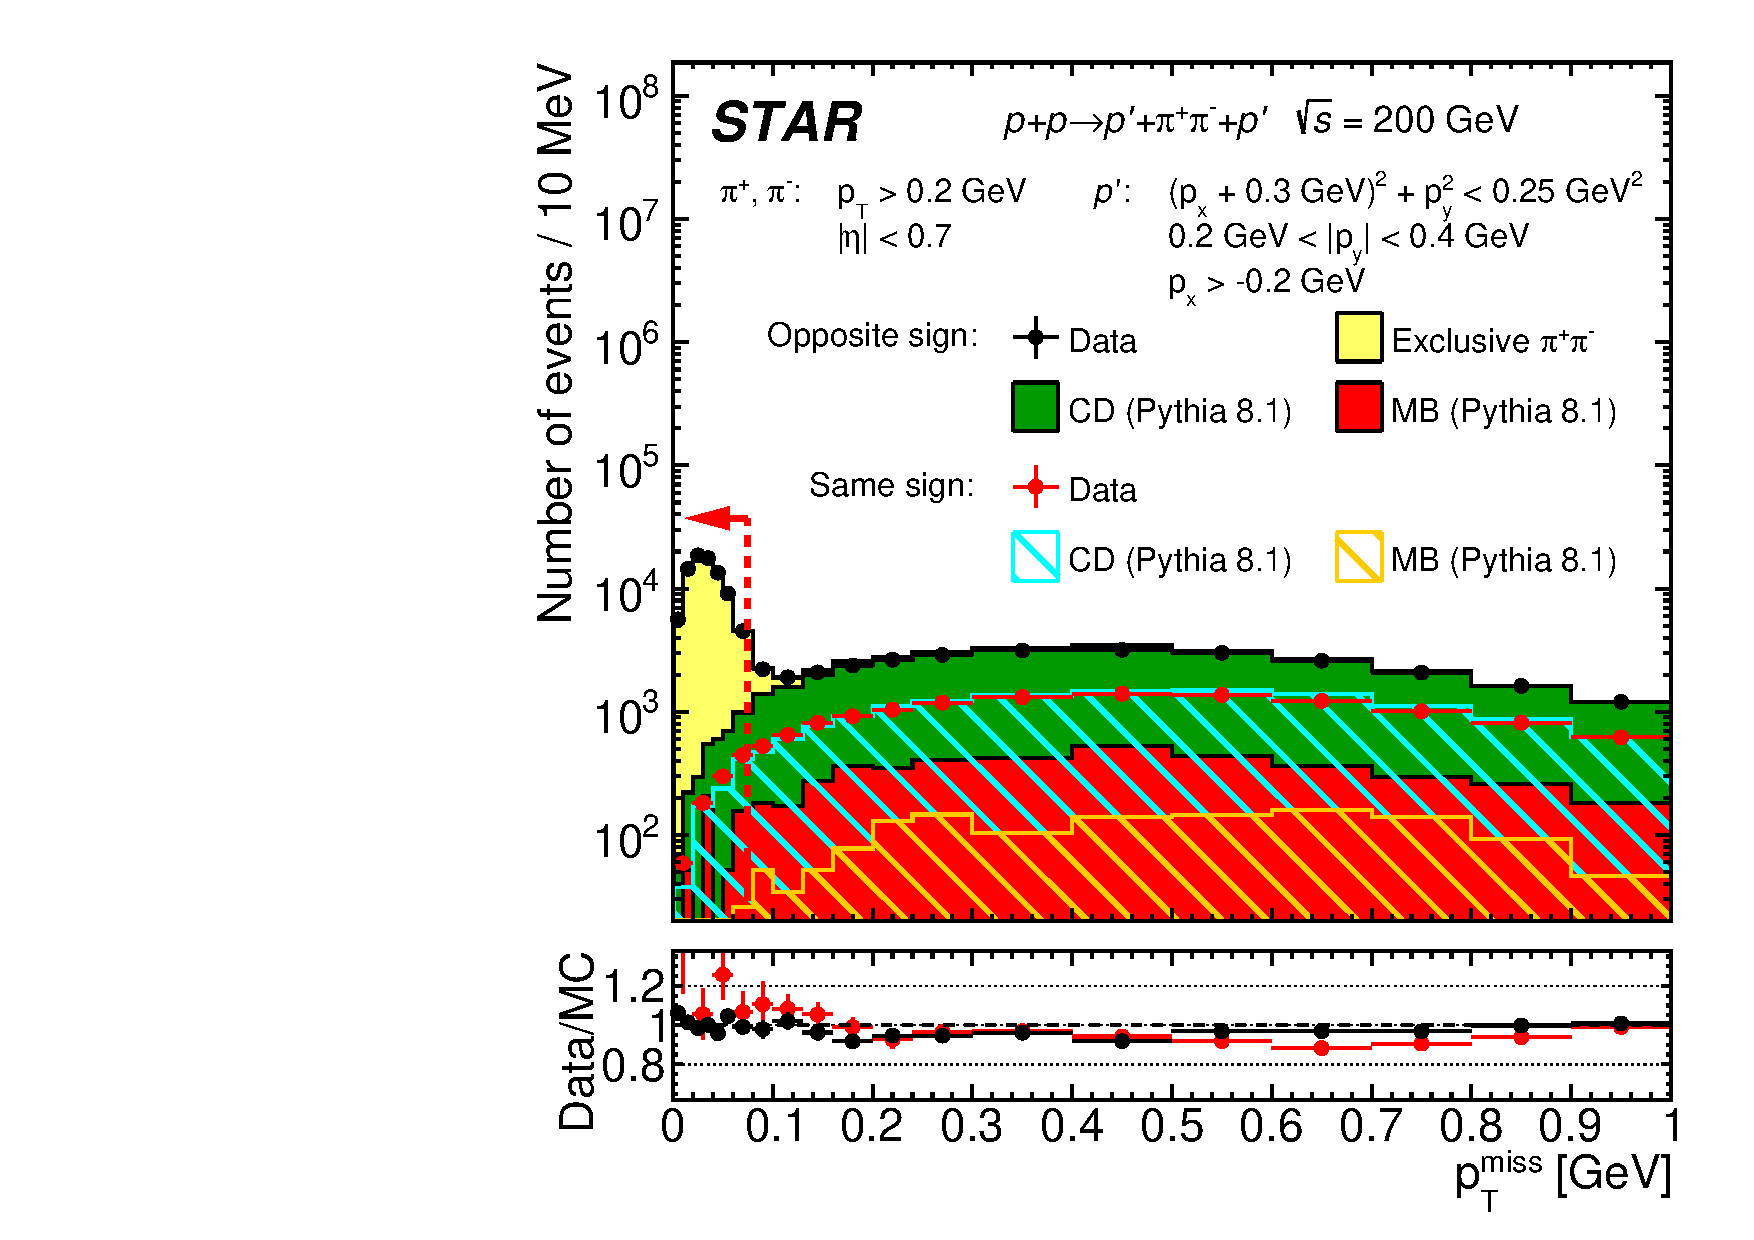
\includegraphics[width=1.05\linewidth,page=1]{graphics/backgrounds/dataVsMc/Ratio_LogY_MissingPt_OppositeAndSameSign.pdf}}
  \end{subfigure}\\
    \begin{minipage}[t][1.042\linewidth][t]{\linewidth}\vspace{20pt}
    \caption[Comparison of $p_{T}^{\text{miss}}$ for CEP $\pi^{+}\pi^{-}$ events between data and embedded MC.]{Comparison of $p_{T}^{\text{miss}}$ for CEP $\pi^{+}\pi^{-}$ events between data and embedded MC after full selection (except cut on presented quantity). Top left and top right plot differ only in the $y$-axis (left: linear, right: logarithmic). In addition to signal channel (opposite-sign particles) also control background channel (same-sign particles) is contained in the plots. Data are represented by black (opposite-sign) or red (same-sign) points, while stacked MC predictions are drawn as filled (opposite-sign) or hatched (same-sign) histograms of different colors. Histogram from each MC process has been normalized according to prescription in the text. Vertical error bars represent statistical uncertainties, horizontal bars represent bin sizes.\\Left bottom plot differ from the top plots in the content of Pythia MCs - in the bottom plot events with $\pi^{\pm}\pi^{\mp}$+neutrals in the central state were preserved, demonstrating significant inconsitency between data and MC in the ratio of opposite-sign to same-sign events if such events are not rejected.}\label{fig:Ratio_MissingPt}%
  \end{minipage}
}%
\end{figure}
%--------------------------- 

